\documentclass{article}


% if you need to pass options to natbib, use, e.g.:
%     \PassOptionsToPackage{numbers, compress}{natbib}
% before loading neurips_2025

% ready for submission
% \usepackage{neurips_2025}


% to compile a preprint version, e.g., for submission to arXiv, add add the
% [preprint] option:
    % \usepackage[preprint]{neurips_2025}


% to compile a camera-ready version, add the [final] option, e.g.:
    \usepackage[final]{neurips_2025}


% to avoid loading the natbib package, add option nonatbib:
%    \usepackage[nonatbib]{neurips_2025}


\usepackage[utf8]{inputenc} % allow utf-8 input
\usepackage[T1]{fontenc}    % use 8-bit T1 fonts
\usepackage{hyperref}       % hyperlinks
\usepackage{url}            % simple URL typesetting
\usepackage{booktabs}       % professional-quality tables
\usepackage{amsfonts}       % blackboard math symbols
\usepackage{nicefrac}       % compact symbols for 1/2, etc.
\usepackage{microtype}      % microtypography
\usepackage{xcolor}         % colors
\usepackage{graphicx}
\usepackage{booktabs, amsthm, amsmath}
\usepackage{algorithm, algpseudocode} % pseudocode
\usepackage{tikz}
\usetikzlibrary{arrows,automata,positioning}
\newcommand{\x}{\mathbf{x}}
\newcommand{\N}{\mathcal{N}}
\newcommand{\mP}{\mathcal{P}}
\newcommand{\E}{\mathbb{E}}
\newcommand{\Var}{\operatorname{Var}}
\newcommand{\Cov}{\operatorname{Cov}}
\newcommand{\Beta}{\operatorname{Beta}}
\newcommand{\Bern}{\operatorname{Bern}}
\newcommand{\argmax}{\mathop{\rm argmax}}

\title{Diffusion for Offline Bandit}


% The \author macro works with any number of authors. There are two commands
% used to separate the names and addresses of multiple authors: \And and \AND.
%
% Using \And between authors leaves it to LaTeX to determine where to break the
% lines. Using \AND forces a line break at that point. So, if LaTeX puts 3 of 4
% authors names on the first line, and the last on the second line, try using
% \AND instead of \And before the third author name.


\author{Xinyue Ying \\
  ShanghaiTech University\\
  2024233224 \\
  \texttt{yingxy2024@shanghaitech.edu.cn} \\
  \And
  Shouchen Zhou \\
  ShanghaiTech University\\
  2021533042 \\
  \texttt{zhoushch@shanghaitech.edu.cn} \\
}


\begin{document}

\maketitle

\begin{abstract}
Offline multi-armed bandit methods are frequently constrained by sparse or distributionally incomplete historical logs. This work introduces discrete diffusion models as principled generators that synthesize additional, distribution-consistent samples to avoid lacking data. We then used the discrete diffusion model in two canonical settings. In the stochastic bandit, a diffusion model fitted to offline trajectories expands the dataset without further interaction; on a newly defined class of non-Bernoulli reward functions where Thompson Sampling is inconsistent, diffusion-augmented logs gathered under UCB still deliver competitive policies. In the contextual bandit, a conditional diffusion model produces arm-specific reward distributions conditioned on context, enabling sampling-based decisions that capture uncertainty beyond the mean. Across both tasks, the discrete diffusion model achieves significant results.
\end{abstract}

\section{Introduction} \label{sec:1_introduction}

\textbf{Diffusion models}\cite{campbell2022continuous} are generative models that learn data distributions through step-by-step denoising. While popular in image generation, they also excel at modeling complex, multimodal structures in other domains.

\begin{center}
    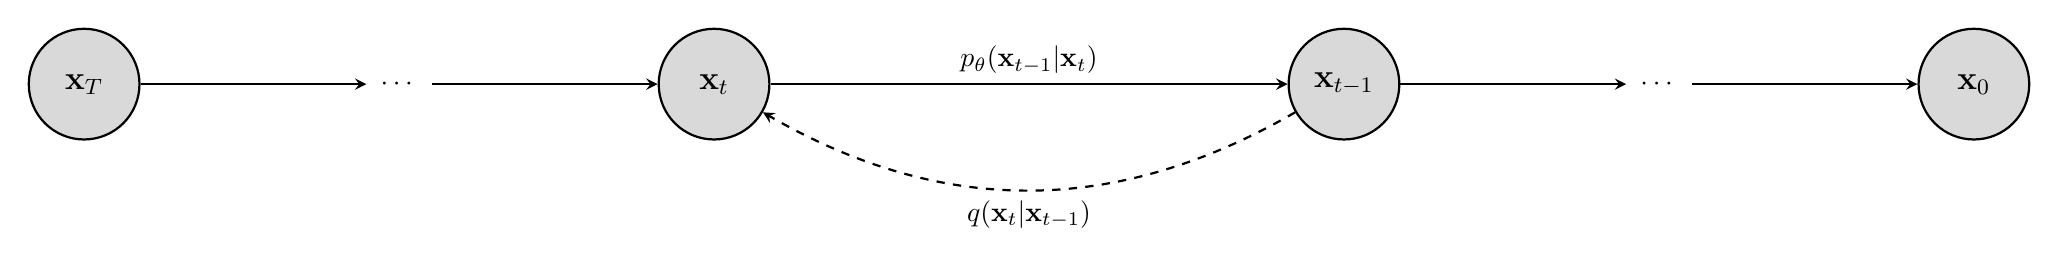
\begin{tikzpicture}[->, >=stealth, auto, thick, node distance=1.5cm]
        \tikzstyle{every state} = [
            fill=gray!30,
            draw=black,
            circle,
            minimum size=40pt,
            font=\large\bfseries
        ]

        \tikzstyle{ellipsis state} = [
            fill=none,
            draw=none,
            circle,
            minimum size=20pt
        ]

        \node[state] (1) {$\x_T$};
        \node[ellipsis state] (ellipsis1) at (4,0) {$\cdots$};
        \node[state] (2) at (8, 0) {$\x_t$};
        \node[state] (3) at (16, 0) {$\x_{t-1}$};
        \node[ellipsis state] (ellipsis2) at (20, 0) {$\cdots$};
        \node[state] (4) at (24, 0) {$\x_0$};

        \draw[->] (1) -- (ellipsis1);
        \draw[->] (ellipsis1) -- (2);

        \draw[->] (2) -- (3) node[midway, above] {$p_{\theta}(\x_{t-1}|\x_t)$};

        \path (3) edge[bend left=30, dashed] node[midway, below] {$q(\x_t|\x_{t-1})$} (2);

        \draw[->] (3) -- (ellipsis2);
        \draw[->] (ellipsis2) -- (4);
    \end{tikzpicture}
    \captionof{figure}{Diffusion model represented as a Markov chain, with a forward process for noise addition during training and a backward process for denoising and generation.}
\end{center}

In this work, we explore diffusion in \textbf{offline bandit learning} from two perspectives: Stochastic Bandit and Contextual Bandit.

\subsection{Stochastic Bandit}
In the stochastic multi-armed bandit setting, a small set of interaction logs can be collected in advance and used as an offline dataset, yielding better initial decisions and shortening the cold-start phase. Yet these logs are often limited in size, lack coverage, and exhibit distributional bias, which constrains policy optimisation. To mitigate these issues, we employ a discrete diffusion model to generate pseudo-samples that match the empirical distribution of the original logs, thereby enlarging the dataset. Specifically, the diffusion model is first trained on the real logs, then used to synthesise additional trajectories, which are merged with the original data to pre-train (or warm-start) the bandit algorithm before a brief online fine-tuning stage. Experiments demonstrate that the diffusion-augmented dataset significantly improves policy quality and accelerates convergence compared with using only the original logs or relying solely on online learning.



\subsection{Contextual Bandit}
The contextual bandit problem is a fundamental framework for sequential decision-making under uncertainty. At each round $t \in \{1, \dots, T\}$, an agent observes a context and selects an action from a finite set. Each action is associated with a feature vector, and upon selection, the agent receives a reward drawn from an unknown distribution conditioned on the context and chosen action. The goal is to maximize the expected cumulative reward over $T$ rounds. 

A common modeling assumption is that the reward can be expressed as the sum of a deterministic mean and an additive noise term: $r = \mathbb{E}[r \mid c, a] + \varepsilon$. Most existing methods focus on estimating the mean $\mathbb{E}[r \mid c, a]$, while treating $\varepsilon$ as an independent and unstructured random variable. This includes classical linear models such as LinUCB \citep{li_contextual-bandit_2010} and LinTS \citep{agrawal_thompson_2014}, kernel-based approaches like GP-UCB \citep{srinivas_gaussian_nodate} and KernelUCB \citep{valko_finite-time_2013}, and deep learning-based models such as NeuralUCB\citep{zhou_neural_2020} and NeuralTS \citep{zhang_neural_2021}. While differing in model class and complexity, these methods share a fundamental reduction of reward modeling to point estimation of the mean and fail to capture important structure in the conditional reward distribution.

However, real-world reward distributions are often multimodal, asymmetric, or heavy-tailed, characteristics that are not captured by simple mean estimators. Risk-sensitive objectives, such as Conditional Value-at-Risk (CVaR) or mean-variance criteria \citep{sani2012risk}, attempt to account for such uncertainties, but they typically rely on handcrafted assumptions and only incorporate limited aspects of the reward distribution. However, these methods do not attempt to learn the full reward distribution itself.


In this work, we propose a new approach to contextual bandits by directly modeling the full reward distribution $P(r \mid c, a)$ using a diffusion-based generative model. This enables us to capture aleatoric uncertainty and richer structure in the reward distribution than conventional estimators allow.
\section{Related Work} \label{sec:2_related_work}

\paragraph{Stochastic Bandit}
The stochastic multi-armed bandit seeks an optimal exploration–exploitation balance over a finite set of arms. Classical solutions include the optimistic Upper Confidence Bound (UCB)~\cite{UCB} family and the Bayesian method Thompson Sampling~\cite{TS}, which couples exploration and exploitation through posterior sampling. In contrast to these confidence-based or posterior-based randomisation schemes, the gradient bandit~\cite{sutton1999policy} directly performs ascent on a parameterised stochastic policy, continuously adapting the arm-selection probabilities.

As large-scale applications raise demands for generalisation and sample efficiency, attention has shifted to offline bandits. When the available logs are small, however, reliance on estimators alone can be unreliable, inspiring the use of generative models to enlarge data coverage: variational autoencoders~\cite{VAE} and GANs~\cite{GAN}, and recently most famous diffusion models~\cite{ddpm} have already been applied to synthesise supplementary samples for offline reinforcement learning. Discrete diffusion models, with their stable training and high sample fidelity, now offer a promising alternative for data augmentation in offline bandits. Following this line, the present study trains a discrete diffusion model on limited interaction logs in the stochastic bandit setting, generates pseudo-trajectories consistent with the empirical distribution, and employs the augmented dataset to warm-start both UCB, Thompson Sampling, and gradient-based algorithms. Experiments confirm that these diffusion-generated samples markedly reduce initial regret and accelerate convergence.



\paragraph{Contextual Bandit}
Contextual bandit algorithms address sequential decision-making problems where, at each round, an agent observes a context, selects an action, and receives a stochastic reward. The aim is to maximize cumulative reward by learning the reward-generating relationship between context-action pairs.  The methods for modeling this relationship have progressively advanced from simple linear formulations to more expressive nonparametric and deep learning-based approaches. In the linear setting, Li et al.\cite{li_contextual-bandit_2010} proposed LinUCB and Agrawal and Goyal \cite{agrawal_thompson_2014} developed LinTS, both of which assume a linear reward model over context-action features and construct confidence bounds around parameter estimates. More general nonlinear bandits without making strong modeling assumptions have also be considered. Srinivas et al.\cite{srinivas_gaussian_nodate} introduced GP-UCB, and Valko et al. \cite{valko_finite-time_2013} proposed KernelUCB, extending the hypothesis class to reproducing kernel Hilbert spaces (RKHS), enabling more expressive reward representations. More recently, neural network-based methods such as NeuralUCB \cite{zhou_neural_2020} and NeuralTS \cite{zhang_neural_2021} have employed deep learning architectures to approximate complex reward functions, incorporating uncertainty through gradient-based proxies or auxiliary variance estimation. Despite these advances, the primary objective of these methods remains unchanged: to estimate the conditional expectation of the reward given context and action, without explicitly modeling the structure of the full reward distribution.
\section{Methods} \label{sec:3_methods}

\subsection{Stochastic Bandit}\label{sec:stochastic_bandit_method}
Policy-based reinforcement learning dispenses with value functions and instead learns the policy directly.  
A parameter vector $\theta$ defines a conditional distribution $\pi_{\theta}(a\mid s)=P(a\mid s;\theta)$, from which an action is sampled at each decision point.  

For a stochastic policy $\pi_{\theta}(a|s)$, it is desirable to decrease the probability of actions that yield low returns and to increase the probability of those that yield high returns. Because the policy is differentiable with respect to $\theta$, such methods enjoy favourable convergence properties and can be optimised efficiently with the policy-gradient technique.

Since the policy is fully determined by $\theta$, whereas state transitions are governed by the environment dynamics,  
the probability of a state–action–reward trajectory
\[\psi=\bigl(s_0,a_0,r_1,\dots,s_{T-1},a_{T-1},r_T,s_T\bigr)\]
depends only on $\theta$. Viewing trajectories as samples of the random variable $\Psi\sim P_{\theta}$, their likelihood is
\[
P_{\theta}(\psi)=\mu(s_0)\prod_{t=0}^{T-1}
\pi_{\theta}(a_t\mid s_t)\,\mathcal{P}^{a_t}_{s_t,s_{t+1}},
\]
where $\mu(s_0)$ is the initial-state distribution and $\mathcal{P}^{a_t}_{s_t,s_{t+1}}$ is the environment’s transition probability. A trajectory’s cumulative reward is
\[
R(\psi)=\sum_{t=1}^{T} r_t.
\]

The learning objective is to find parameters $\theta$ that maximise the expected return
\[
J(\theta)=
\mathbb{E}_{\Psi\sim P_{\theta}}\!\bigl[R(\Psi)\bigr]
=\sum_{\psi}P_{\theta}(\psi)R(\psi),
\]
leading to the unconstrained optimisation problem $\max_{\theta}J(\theta)$.  
Gradient ascent is standard, with
\[
\begin{aligned}
\nabla_{\theta}J(\theta)
&= \nabla_{\theta}\sum_{\psi}P_{\theta}(\psi)R(\psi)\\
&= \sum_{\psi}P_{\theta}(\psi)R(\psi)\,\nabla_{\theta}\log P_{\theta}(\psi)\\
&= \mathbb{E}_{\Psi\sim P_{\theta}}\!\Bigl[
  R(\Psi)\sum_{t=0}^{T-1}\nabla_{\theta}\log\pi_{\theta}(A_t\mid S_t)
\Bigr]\\
&\approx \frac{1}{m}\sum_{i=1}^{m}
  R(\psi_i)\sum_{t=0}^{T-1}
  \nabla_{\theta}\log\pi_{\theta}(a_t^{\,i}\mid s_t^{\,i}),
\end{aligned}
\]
where the approximation uses $m$ sampled trajectories
\[
\psi_i=\bigl(s_0^{\,i},a_0^{\,i},r_1^{\,i},\dots,
            s_{T-1}^{\,i},a_{T-1}^{\,i},r_T^{\,i},s_T^{\,i}\bigr),
\]
and $\nabla_{\theta}\log\pi_{\theta}(a_t^{\,i}\mid s_t^{\,i})$ is the score function.  
With an offline trajectory dataset, this estimator enables direct optimisation of $\theta$, yielding a high-quality initial policy that can later be refined online.

Although unbiased, the estimator often has high variance.  
Introducing a state-dependent baseline $b(s_t)$ preserves unbiasedness while reducing variance, giving
\[
\nabla_{\theta}J(\theta)\approx
\frac{1}{m}\sum_{i=1}^{m}\sum_{t=0}^{T-1}
\bigl[(R_t^{\,i}-b_t(s_t^{\,i}))\,
      \nabla_{\theta}\log\pi_{\theta}(a_t^{\,i}\mid s_t^{\,i})\bigr].
\]

In summary, policy-gradient reinforcement learning maximises the expected return of trajectories contained in an offline dataset, directly optimising a parameterised policy without extra interaction and providing a strong starting point for subsequent learning.

Similar to policy-gradient methods in reinforcement learning, a stochastic multi-armed bandit can be viewed as a special case of reinforcement learning in which the state remains unchanged after each action; effectively, the system contains only a single dummy state. Under this assumption, the usual state variable $s$ and the transition probabilities $\mathcal{P}_{s,s'}^{a}$ degenerate to constants and can be ignored.  
Consequently, a state–action–reward trajectory reduces to an action–reward sequence
\[
\psi=\bigl(a_0,r_1,\dots,a_{T-1},r_T\bigr).
\]
Each trajectory $\psi$ is a sample of the random variable $\Psi\sim P_{\theta}$.  
Because every action choice may depend on all previous actions and their received rewards, the probability of observing $\psi$ is
\[
P_{\theta}(\psi)=
\prod_{t=0}^{T-1}
\pi_{\theta}\!\bigl(a_t \mid a_0,r_1,\ldots,a_{t-1},r_t\bigr).
\]

The objective is defined analogously as
\[
J(\theta)=
\mathbb{E}_{\Psi\sim P_{\theta}}\!\bigl[R(\Psi)\bigr]
=\sum_{\psi}P_{\theta}(\psi)R(\psi).
\]

In a stochastic bandit, the policy is parameterised by the softmax of a preference function,
\[
\pi_{\theta}(a)=
\frac{\exp\!\bigl(\beta_t H_{\theta}(a)\bigr)}
{\sum_{a'}\exp\!\bigl(\beta_t H_{\theta}(a')\bigr)},
\]
So its gradient can be written as
\[
\begin{aligned}
\nabla_{\theta}\log\pi_{\theta}\!\bigl(a_t^i\bigr)
&=
\nabla_{\theta}\log
\frac{\exp\!\bigl(\beta_t H_{\theta}
(a_t^i \mid a_0^i, r_1^i,\ldots,a_{t-1}^i,r_t^i)\bigr)}
{\displaystyle
\sum_{a}\exp\!\bigl(\beta_t H_{\theta}
(a \mid a_0^i, r_1^i,\ldots,a_{t-1}^i,r_t^i)\bigr)}
\\[4pt]
&=
\beta_t\nabla_{\theta}
H_{\theta}\!\bigl(a_t^i \mid a_0^i, r_1^i,\ldots,a_{t-1}^i,r_t^i\bigr)
\\
&\quad-
\beta_t\frac{\displaystyle
\sum_{a}\nabla_{\theta}H_{\theta}
(a \mid a_0^i, r_1^i,\ldots,a_{t-1}^i,r_t^i)
\exp\!\bigl(\beta_t H_{\theta}(a \mid a_0^i, r_1^i,\ldots,a_{t-1}^i,r_t^i)\bigr)}
{\displaystyle
\sum_{a}\exp\!\bigl(\beta_t H_{\theta}
(a \mid a_0^i, r_1^i,\ldots,a_{t-1}^i,r_t^i)\bigr)}
\\[4pt]
&=
\beta_t\!\Bigl(
\nabla_{\theta}H_{\theta}\!\bigl(a_t^i \mid a_0^i, r_1^i,\ldots,a_{t-1}^i,r_t^i\bigr)
-\sum_{a}\pi_{\theta}(a)\,
\nabla_{\theta}H_{\theta}
(a \mid a_0^i, r_1^i,\ldots,a_{t-1}^i,r_t^i)
\Bigr),
\end{aligned}
\]
where the exact form of
$\nabla_{\theta}H_{\theta}
(a\mid a_0^i, r_1^i,\ldots,a_{t-1}^i,r_t^i)$
depends on the chosen preference function $H_{\theta}(a)$.

Accordingly, the policy gradient for the multi-armed bandit becomes
\[
\begin{aligned}
\nabla_{\theta}J(\theta)
&\approx
\frac{1}{m}\sum_{i=1}^{m}\sum_{t=0}^{T-1}
\Bigl[(R_t^i-b_t)\,
\nabla_{\theta}\log\pi_{\theta}
\bigl(a_t^i \mid a_0^i, r_1^i,\ldots,a_{t-1}^i,r_t^i\bigr)\Bigr]
\\
&=
\frac{1}{m}\sum_{i=1}^{m}\sum_{t=0}^{T-1}
\Bigl[(R_t^i-b_t)\,\beta_t\!
\Bigl(
\nabla_{\theta}H_{\theta}\!\bigl(a_t^i \mid a_0^i, r_1^i,\ldots,a_{t-1}^i,r_t^i\bigr)
\\
&\qquad
-\sum_{a}\pi_{\theta}(a)\,
\nabla_{\theta}H_{\theta}
(a \mid a_0^i, r_1^i,\ldots,a_{t-1}^i,r_t^i)
\Bigr)\Bigr].
\end{aligned}
\]

Because the state is fixed in a stochastic bandit, $b_t$ is typically set to a constant or to the running average reward $\bar{R}_t=\tfrac{1}{t}\sum_{\tau=0}^{t-1}R_{\tau}$.  
Moreover, the preference at time $t$ depends on the preference at time $t-1$ together with $(a_{t-1},r_t)$.  
Hence, unlike the Markov decision process setting, the bandit policy gradient cannot be further simplified using causality or Markov properties.

After getting the policy gradient, we can pre-train the stochastic bandit with the given offline dataset in the following alrotihm procedure:
\begin{algorithm}[H]
    \textbf{Input:} the original (unaugmented) offline dataset
    \begin{algorithmic}[1]
      \State Generate additional trajectories with the offline diffusion model to obtain an augmented dataset
      \State Pre-train UCB, Thompson Sampling, policy-gradient, and related algorithms on the augmented dataset
      \State Deploy the pretrained models for online interaction and update the parameters continually
    \end{algorithmic}
    \label{alg:stochastic_bandit_pretrained}
    \caption{Stochastic multi-armed bandit algorithm that augments an offline dataset with trajectories generated by a discrete diffusion model}
\end{algorithm}


\subsection{Contextual Bandit}
We consider the stochastic $K$-armed contextual bandit problem. At each round $t \in [T]$, the agent observes a set of context vectors $\{\mathbf{x}_{t,a} \in \mathbb{R}^d \mid a \in [K]\}$, selects an action $a_t$, and receives a scalar reward $r_{t,a_t} \in \mathbb{R}$. The goal is to design a decision rule that leverages the full reward distribution to make informed and robust choices.
Our goal is to maximize the following pseudo regret:

$$
R_T = \mathbb{E}\left[\sum_{t=1}^T \left( r_{t,a_t^\dagger} - r_{t,a_t} \right)\right],
$$

where the oracle action $a_t^\dagger$ is defined as:
$
a_t^\dagger = \arg\max_{a \in [K]} \pi^*(a \mid \mathbf{x}_{t,a}), 
$
and $\pi^*(a \mid \mathbf{x}_{t,a})$ represents an optimal decision rule that can depend on more than just the mean reward—e.g., variance, risk profiles, or quantiles.

Rather than approximating $\mathbb{E}[r \mid \mathbf{x}, a]$, we adopt a distributional perspective and directly model the full conditional reward distribution:
$
r \sim P(r \mid \mathbf{x}, a). 
$

This allows our method to capture both the central tendency and the uncertainty structure (aleatoric) inherent in the environment, which is crucial in high-stakes or risk-sensitive applications.

\paragraph{Diffusion-Based Reward Sampling}
To capture the full conditional reward distribution $P(r \mid \mathbf{x}, a)$, we employ a diffusion as a flexible generative framework. Given an offline dataset $\mathcal{D}_{\text{offline}} = \{(\mathbf{x}_i, a_i, r_i)\}_{i=1}^N$, the diffusion model is trained to approximate the distribution of rewards conditioned on context-action pairs:

$$
r \sim P_{\text{diff}}(r \mid \mathbf{x}, a; \mathcal{W}_{\text{diff}}), 
$$

where $\mathcal{W}_{\text{diff}}$ denotes the parameters of the learned reverse process. The model consists of a Markovian forward process that gradually adds noise to reward samples, and a learned reverse process that denoises the corrupted inputs to recover samples from the target conditional distribution.

At each round $t$, the agent observes the contextual features $\{\mathbf{x}_{t,a}\}_{a=1}^K$, and for each action $a \in [K]$, it draws a synthetic reward sample $\tilde{r}_a \sim P_{\text{diff}}(r \mid \mathbf{x}_{t,a})$. The action is then selected via:

$$
a_t = \arg\max_{a \in [K]} \tilde{r}_a. 
$$

This sampling-based decision rule inherently reflects the uncertainty encoded in the full reward distribution and allows the agent to balance exploitation and stochastic exploration without requiring explicit posterior variance estimation.

\section{Experiments} \label{sec:4_experiments}


\subsection{Stochastic Bandit}

Using the methods metioned in \ref{sec:stochastic_bandit_method}, the relationship between average regret and the number of rounds for different trajectory-generation methods and algorithms is presented in Figure \ref{fig:stochastic_bandit_pretrained} and Table \ref{table:stochastic_bandit_pretrained}. Each experiment was run for 50000 rounds and repeated 100 times; the regret from each run was averaged cumulatively, and this average is reported as the final result.

\begin{figure}[htbp]
    \centering
    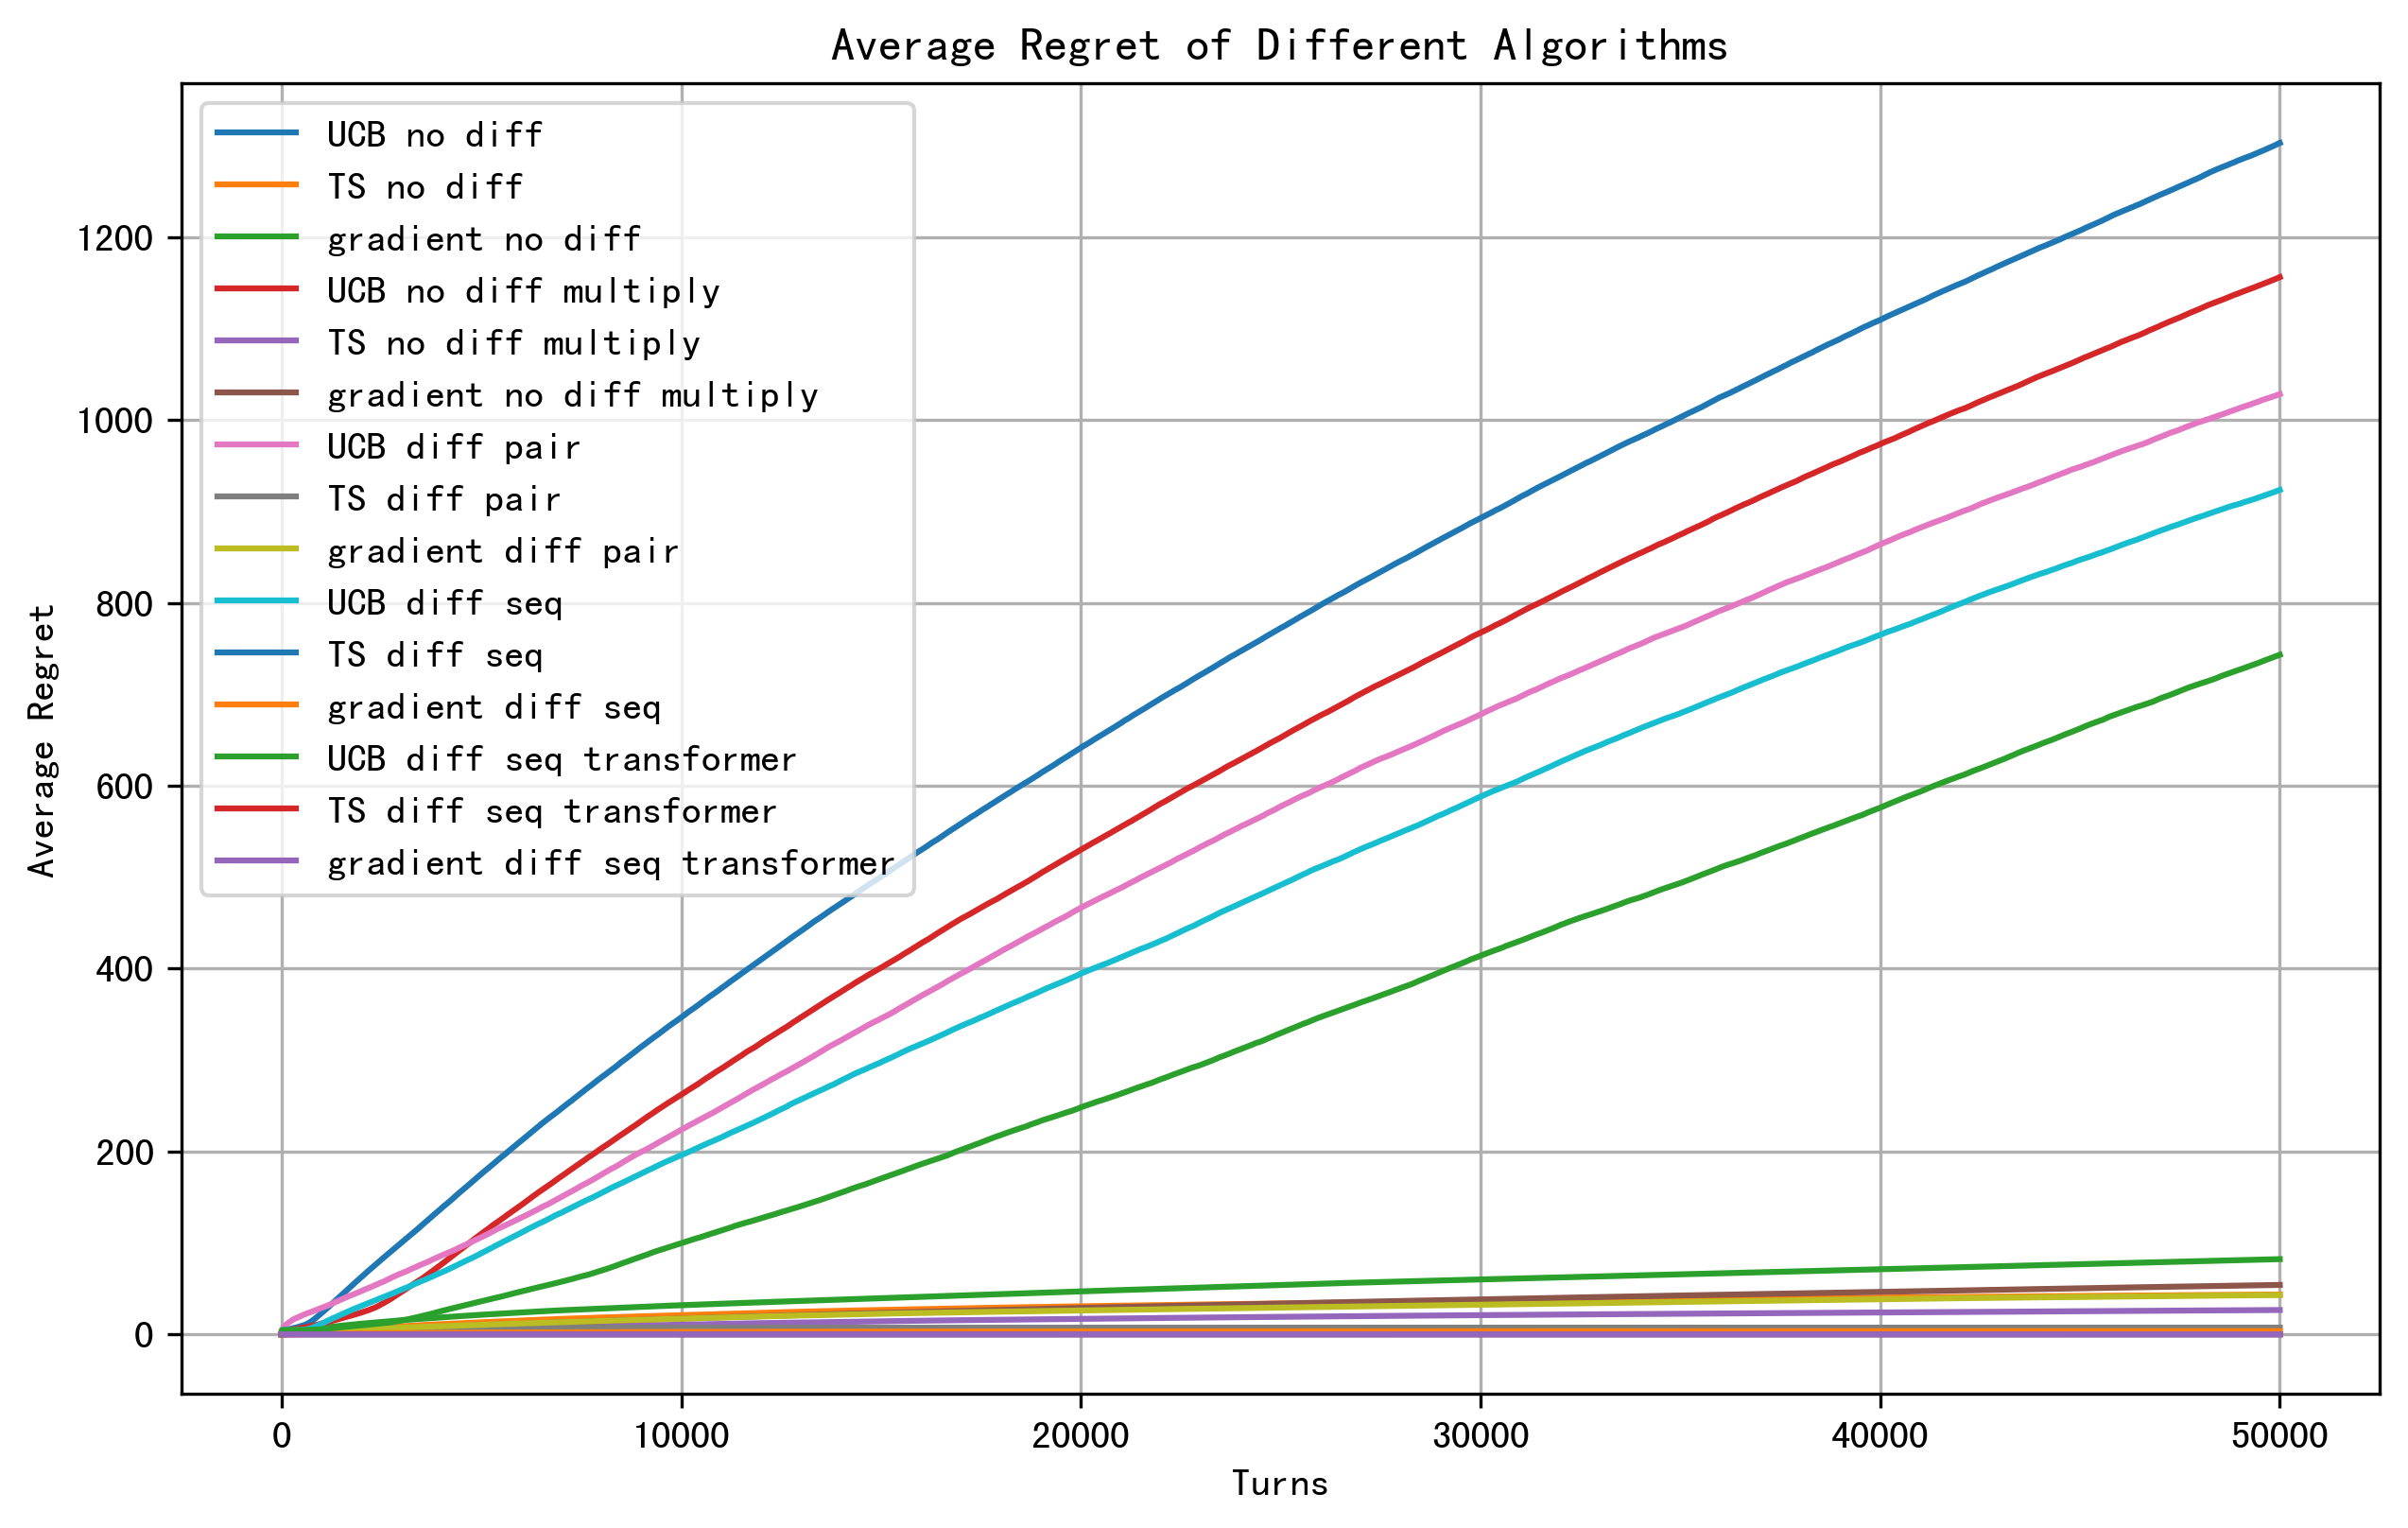
\includegraphics[width=\textwidth]{./Img/stochastic_bandit/pretrain.png}
    \caption{Average cumulative-regret curves for the UCB algorithm (UCB), Thompson Sampling (TS), and the policy-gradient algorithm (gradient) under five data settings: the unaugmented offline dataset (no diff), a duplicated-concatenated version of the original dataset (no-diff-multiply), tuple-level discrete-diffusion augmentation (diff pair), sequence-level discrete-diffusion augmentation (diff seq), and Transformer-based sequence discrete-diffusion augmentation (diff seq transformer).}
    \label{fig:stochastic_bandit_pretrained}
\end{figure}

\begin{table}[htbp]
    \centering
    \begin{tabular}{c c c c}
    \toprule
    Trajectory generation policy & UCB & TS & policy gradient \\
    \midrule
    no offline dataset & 1691.827 & 163.483 & 858.794 \\
    offline, no enlarge & 1303.405 & 43.550  & 82.254 \\
    offline+copy & 1156.635 & 26.596  & 54.048 \\
    offline+diffuse pair & 1028.613 & 7.296 & 42.993 \\
    offline+diffusion sequence & 923.779 & 0.071 & 3.522 \\
    offline+diffusion sequence (Transformer) & 743.441 & 0.008 & 0.002 \\
    \bottomrule
\end{tabular}
\caption{Performance(average accumulated regret) of various algorithms on Bernoulli-reward bandits under different offline-dataset enlargement (trajectory-generation) policies.}
\label{table:stochastic_bandit_pretrained}
\end{table}

We observe that both Thompson Sampling and the policy-gradient algorithm achieve lower regret than UCB. With effective trajectory augmentation, the two methods essentially identify the optimal arm, driving the cumulative regret toward zero. To verify that a discrete-diffusion model can generate additional useful trajectories and thereby improve UCB as well, we varied the amount of synthetic data used for pre-training. All synthetic trajectories were produced with the most effective method identified earlier—the Transformer-based sequence discrete-diffusion model—generating an extra 100, 500, and 1000 trajectories. As baselines of the same sizes, the original (non-diffusion) dataset was duplicated once, five times, and ten times, respectively. Following the same algorithmic procedure, the resulting average-regret curves over rounds for the different generation strategies and algorithms are reported in Figure \ref{fig:stochastic_bandit_num} and Table \ref{table:stochastic_bandit_num}. Each experiment consisted of 50000 rounds, repeated 100 times; the regret values from each run were averaged to obtain the final results.

\begin{figure}[htbp]
    \centering
    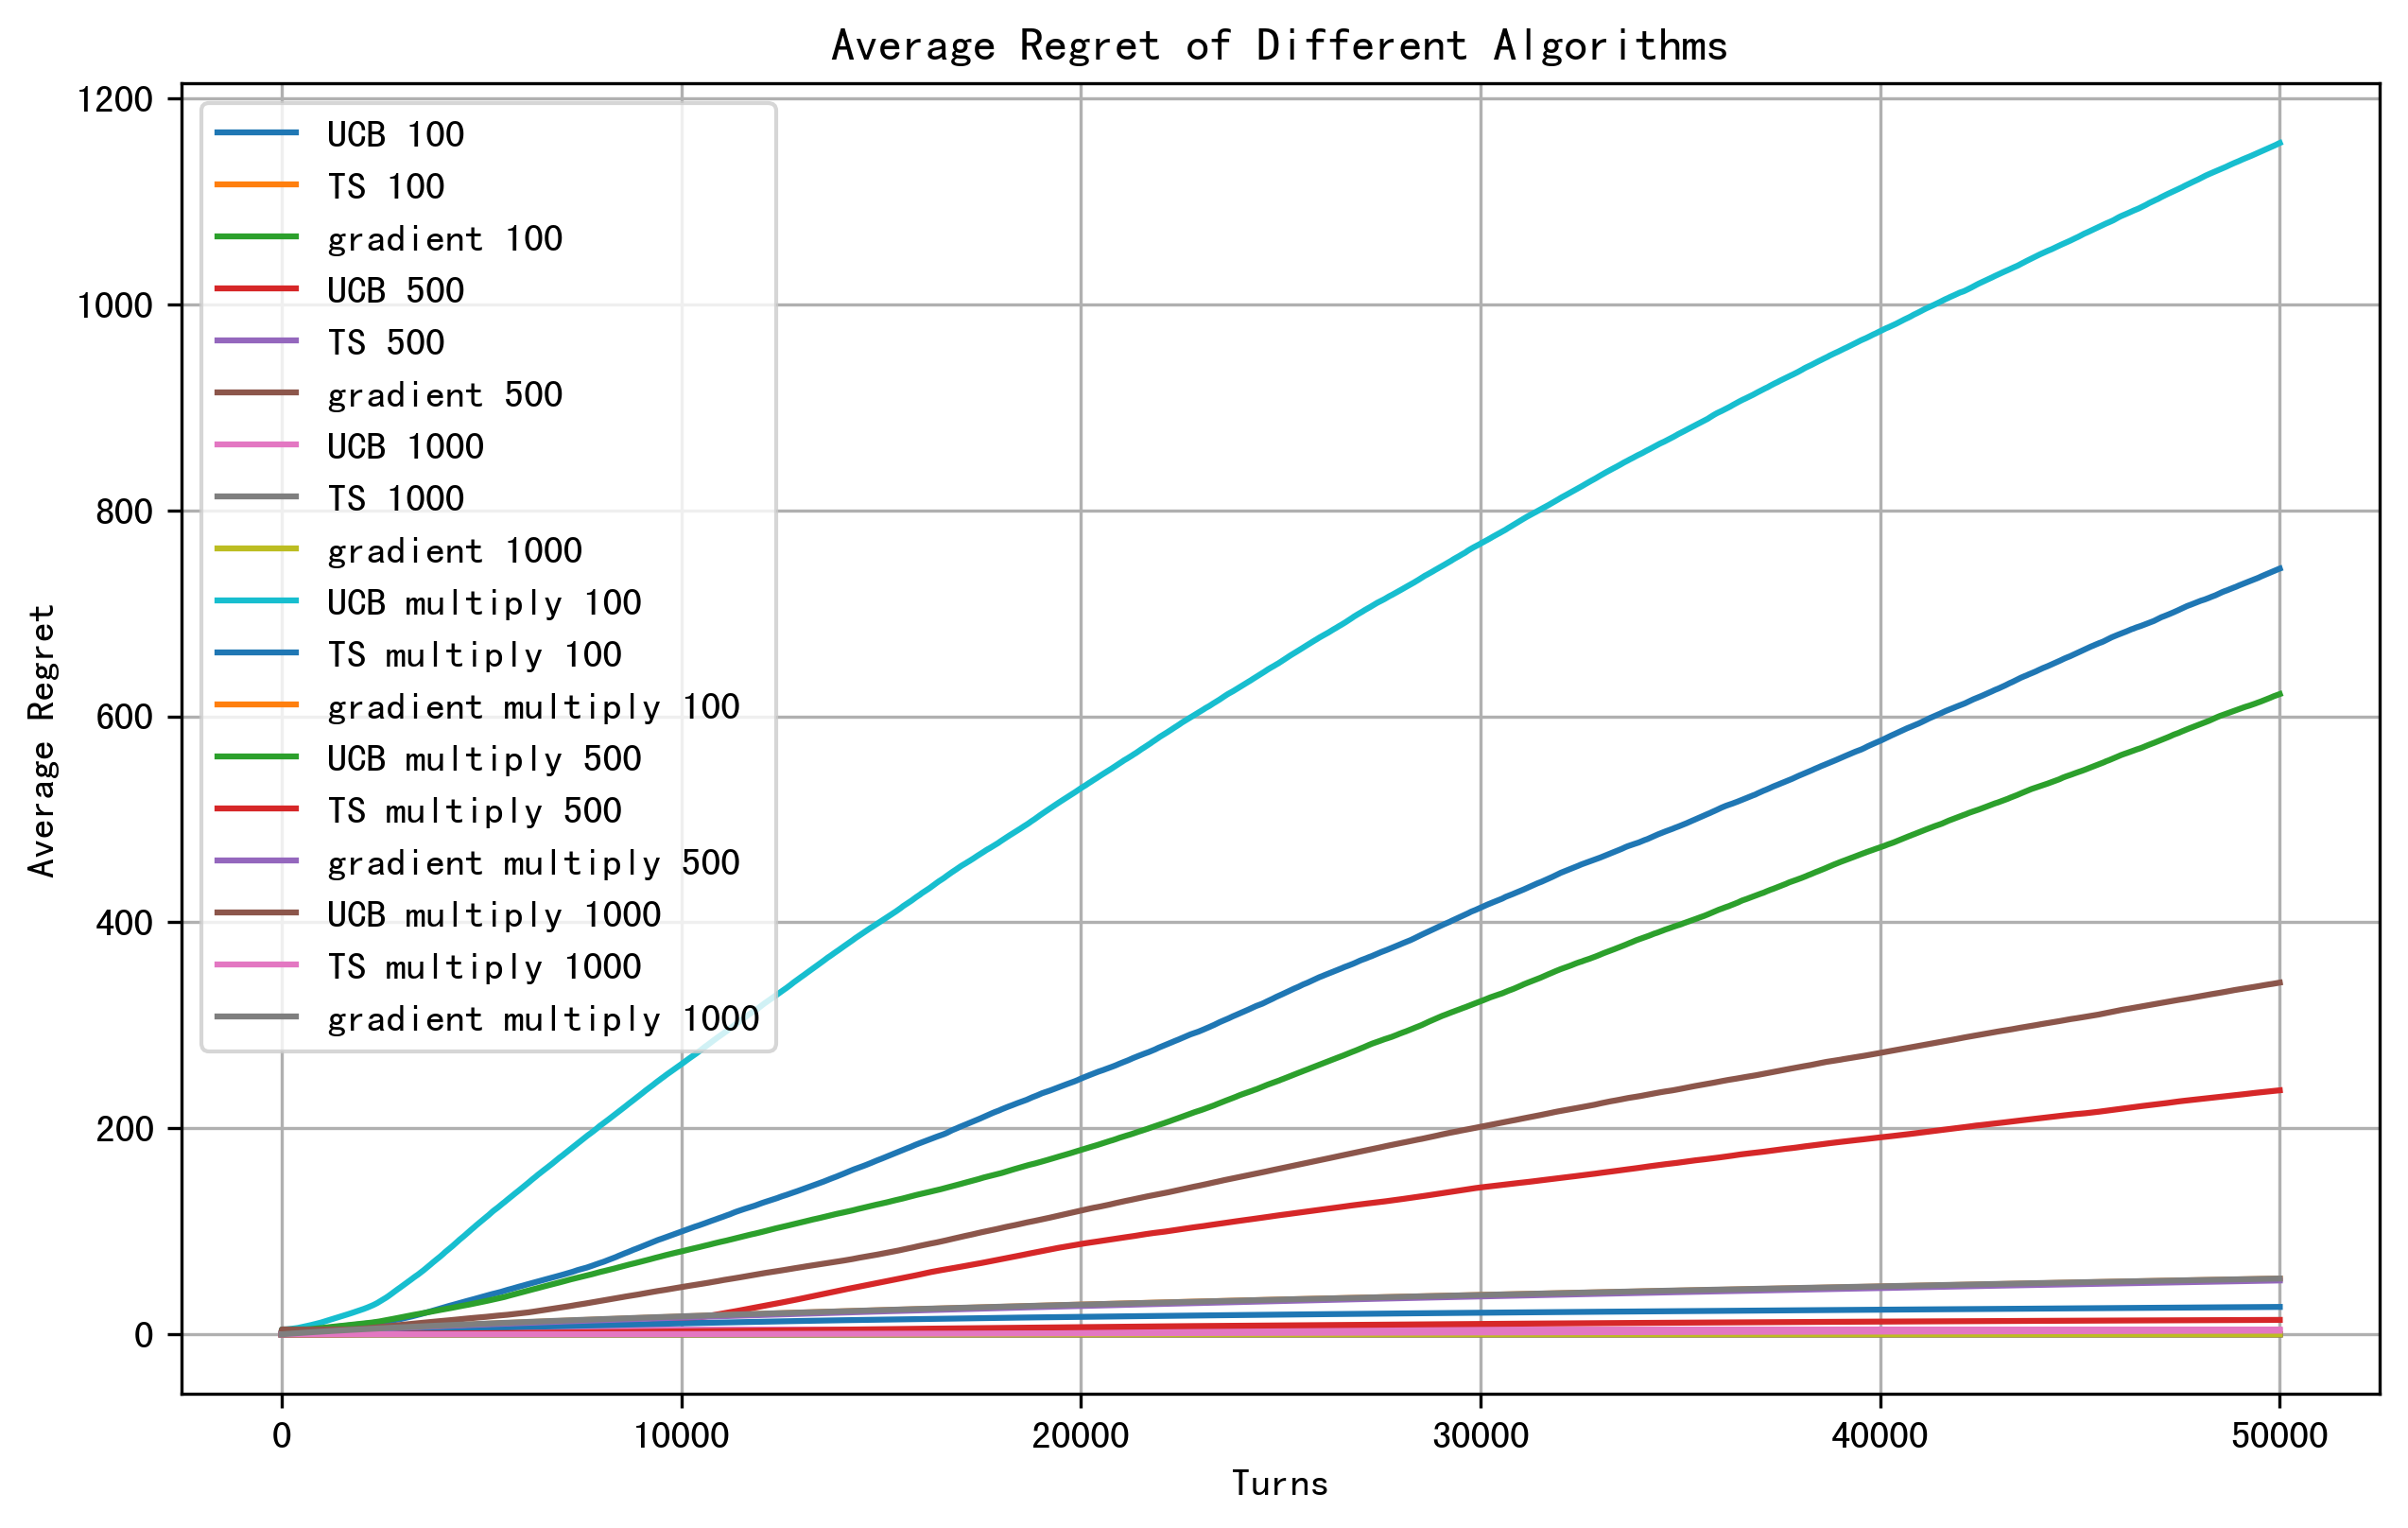
\includegraphics[width=\textwidth]{./Img/stochastic_bandit/time_comparison.png}
    \caption{Average cumulative-regret curves for the UCB algorithm (UCB), Thompson Sampling (TS), and the gradient bandit (gradient) under six data regimes: Transformer-based sequence discrete-diffusion augmentation with 100, 500, and 1 000 additional trajectories (100, 500, 1000) and simple duplication of the original dataset yielding the same numbers of extra trajectories (multiply 100, multiply 500, multiply 1000).}
    \label{fig:stochastic_bandit_num}
\end{figure}

\begin{table}[htbp]
    \centering
    \begin{tabular}{c c c c}
    \toprule
    Trajectory generation policy & UCB & TS & policy gradient \\
    \midrule
    copy, 100 trajectories& 1156.635 & 26.596 & 54.048 \\
    copy, 500 trajectories& 621.581 & 13.996 & 52.293 \\
    copy, 1000 trajectories & 341.470 & 3.517 & 54.164 \\
    diffusion, 100 trajectories & 743.441 & 0.008 & 0.002 \\
    diffusion, 500 trajectories & 236.908 & 0.056 & 0.000 \\
    diffusion, 1000 trajectories & 4.660 & 0.025 & 0.000 \\
    \bottomrule
\end{tabular}
\caption{Performance(average accumulated regret) of various algorithms on Bernoulli-reward bandits under different offline-dataset enlargement (trajectory-generation) policies.}
\label{table:stochastic_bandit_num}
\end{table}

The experimental results indicate that, under identical settings, enlarging the number of trajectories produced by the discrete diffusion model yields substantial gains for all three algorithms—UCB, Thompson Sampling, and the gradient bandit. In particular, both Thompson Sampling and the gradient method converge rapidly once pre-training is introduced, driving their cumulative regret close to zero and underscoring the pivotal role of pre-training in policy learning. The UCB algorithm likewise benefits markedly: its performance improves steadily as more synthetic trajectories are added. A further comparison confirms the effectiveness of discrete diffusion for generating high-quality data: when the number of additional trajectories is held constant, datasets augmented by diffusion outperform those expanded by simply duplicating and concatenating the original logs, demonstrating superior practical utility and generalisation capacity in data-augmentation scenarios.


To evaluate the method’s adaptability under non-ideal reward conditions, we construct a discrete-reward environment in which each arm follows a Bernoulli distribution. Under this setting, Thompson Sampling no longer enjoys a convenient conjugate prior and thus cannot be applied directly. Instead, trajectories are generated by running the UCB algorithm online with the environment, collecting 100 trajectories of length 50. The reward variable is defined as follows:
$$X=\begin{cases}
0 & \text{ w.p. } \theta_1 \\
0.5 & \text{ w.p. } \theta_2 \\
1 & \text{ w.p. } 1-\theta_1-\theta_2 \\
\end{cases}$$

Under three arm-count configurations (20, 25, and 30), we systematically evaluated the effect of diffusion-generated trajectories on the pre-training phase of these algorithms to assess the method’s generalization capability in high-complexity policy spaces.

The discrete diffusion method that demonstrated the best performance under Bernoulli rewards was used to generate 500 additional trajectories. We compared three pre-training strategies: no pre-training, pre-training on the original offline dataset, and pre-training on the offline dataset augmented with these 500 diffusion-generated trajectories. Both the UCB algorithm and a policy-gradient method were evaluated. Following this procedure, the evolution of average regret over rounds for each trajectory-generation method and algorithm is presented in Figure \ref{fig:non_bern} and Table \ref{table:non_bern}. Each experiment ran for 50 000 rounds and was repeated 100 times; the reported results are the average regret across all trials.

\begin{figure}[htbp]
    \centering
    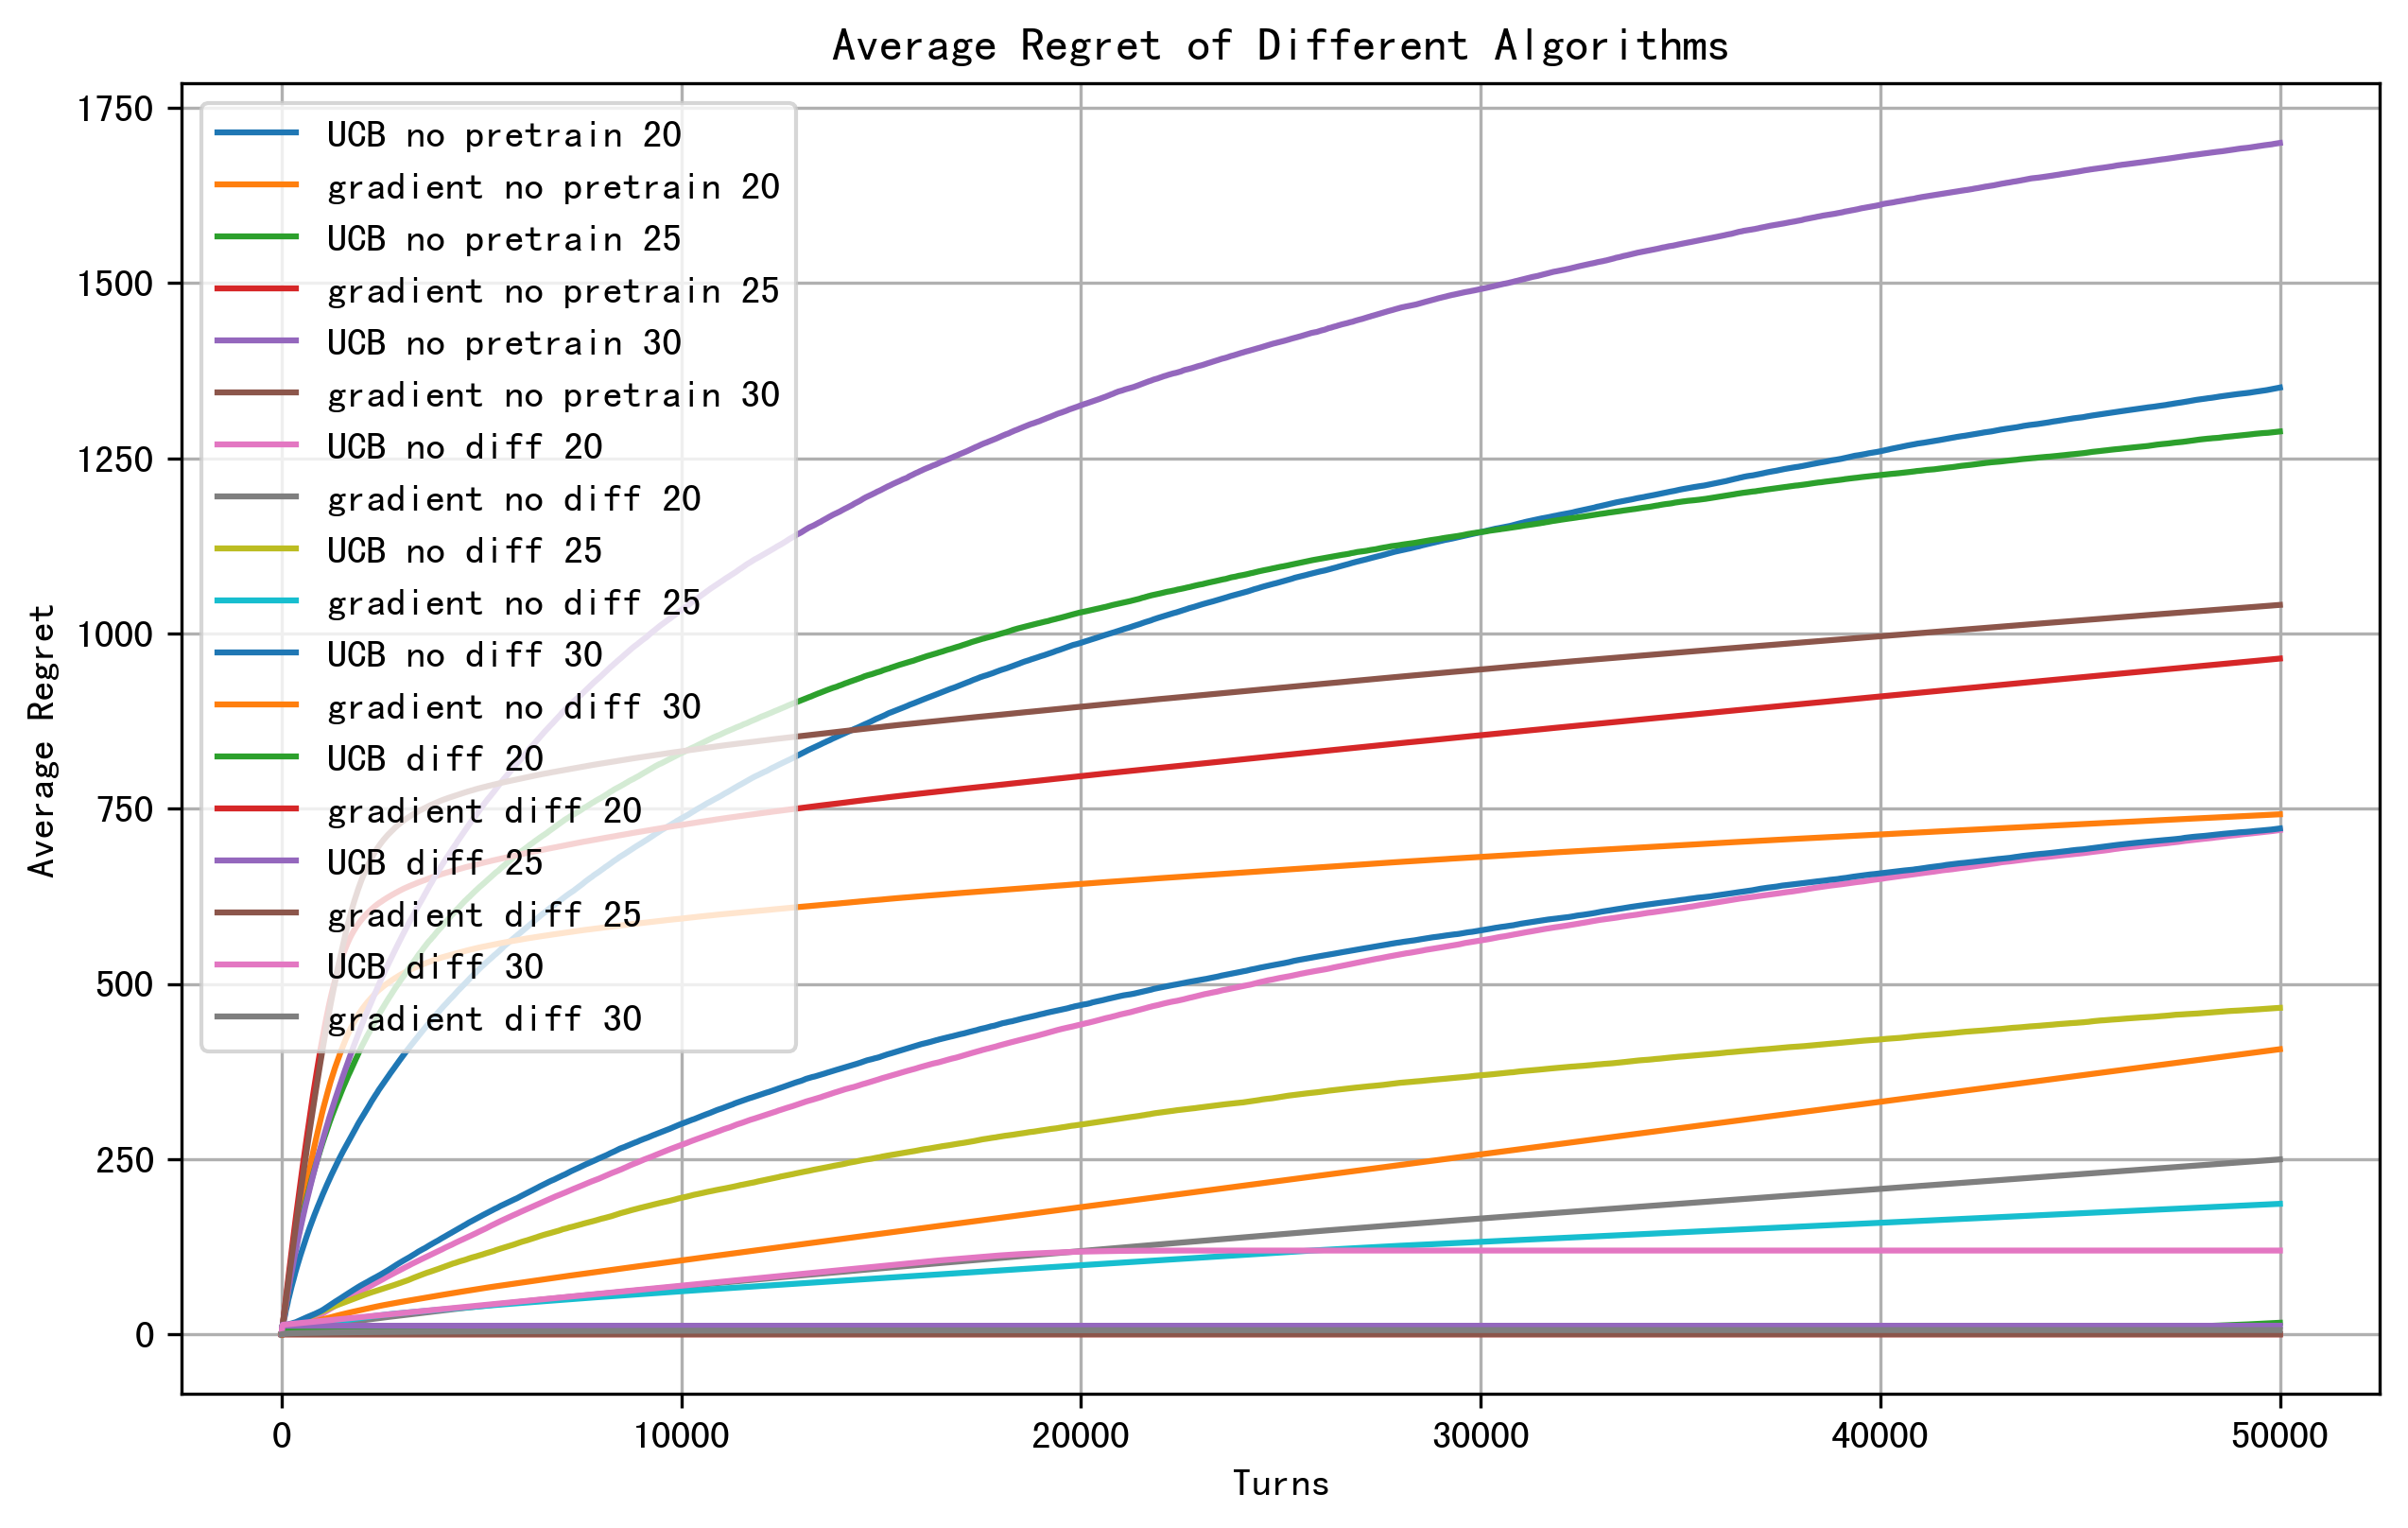
\includegraphics[width=0.97\textwidth]{./Img/stochastic_bandit/non_bern.png}
    \caption{Average cumulative-regret curves for the UCB algorithm (UCB) and the policy-gradient algorithm (Gradient) under nine configurations formed by three arm counts (20, 25, and 30) and three pre-training regimes: no pretraining (no pretrain), pretraining on the original dataset without diffusion (no diff), and pretraining on a dataset augmented with trajectories generated by the Transformer-based sequential discrete diffusion method (diff).}
    \label{fig:non_bern}
\end{figure}

\begin{table}[htbp]
    \centering
    \begin{tabular}{c c c}
    \toprule
    Trajectory generation policy & UCB & policy gradient \\
    \midrule
    no offline dataset, 20 arms & 1351.033 & 742.086 \\
    offline, no enlarge, 20 arms & 719.629 & 249.610 \\
    offline+diffusion sequence (Transformer), 20 arms & 16.517 & 0.000 \\
    no offline dataset, 25 arms & 1288.369 & 964.330 \\
    offline, no enlarge, 25 arms & 465.870 & 186.230 \\
    offline+diffusion sequence (Transformer), 25 arms & 12.220 & 0.000 \\
    no offline dataset, 30 arms & 1700.104 & 1040.903 \\
    offline, no enlarge, 30 arms & 721.866 & 406.857 \\
    offline+diffusion sequence (Transformer), 30 arms & 119.548 & 6.077 \\
    \bottomrule
\end{tabular}
\caption{Performance(average accumulated regret) of various algorithms on Bernoulli-reward bandits under different offline-dataset enlargement (trajectory-generation) policies.}
\label{table:non_bern}
\end{table}

The experimental results indicate that in discrete-reward environments with non-Bernoulli distributions, using UCB-generated online interaction data as trajectories and augmenting the offline dataset via a discrete diffusion model enables both the policy-gradient algorithm and the UCB algorithm to achieve effective performance with 20, 25, and 30 arms. Moreover, as the number of arms increases, a larger volume of trajectory data is required to accurately learn each arm’s reward function.

Since the policy‐gradient algorithm and the gradient bandit algorithm share similar implementations but rest on different principles, we conducted experiments to verify that, when supplied with an offline dataset, the policy‐gradient method yields superior performance. Both algorithms were evaluated under various offline data regimes, and the evolution of their average regret over rounds is shown in Figure \ref{fig:compare_gradient_bandit} and Table \ref{table:compare_gradient_bandit}. Each experiment comprised 50000 rounds and was repeated 100 times; the reported results are the average regret across all runs.

\begin{figure}[htbp]
    \centering
    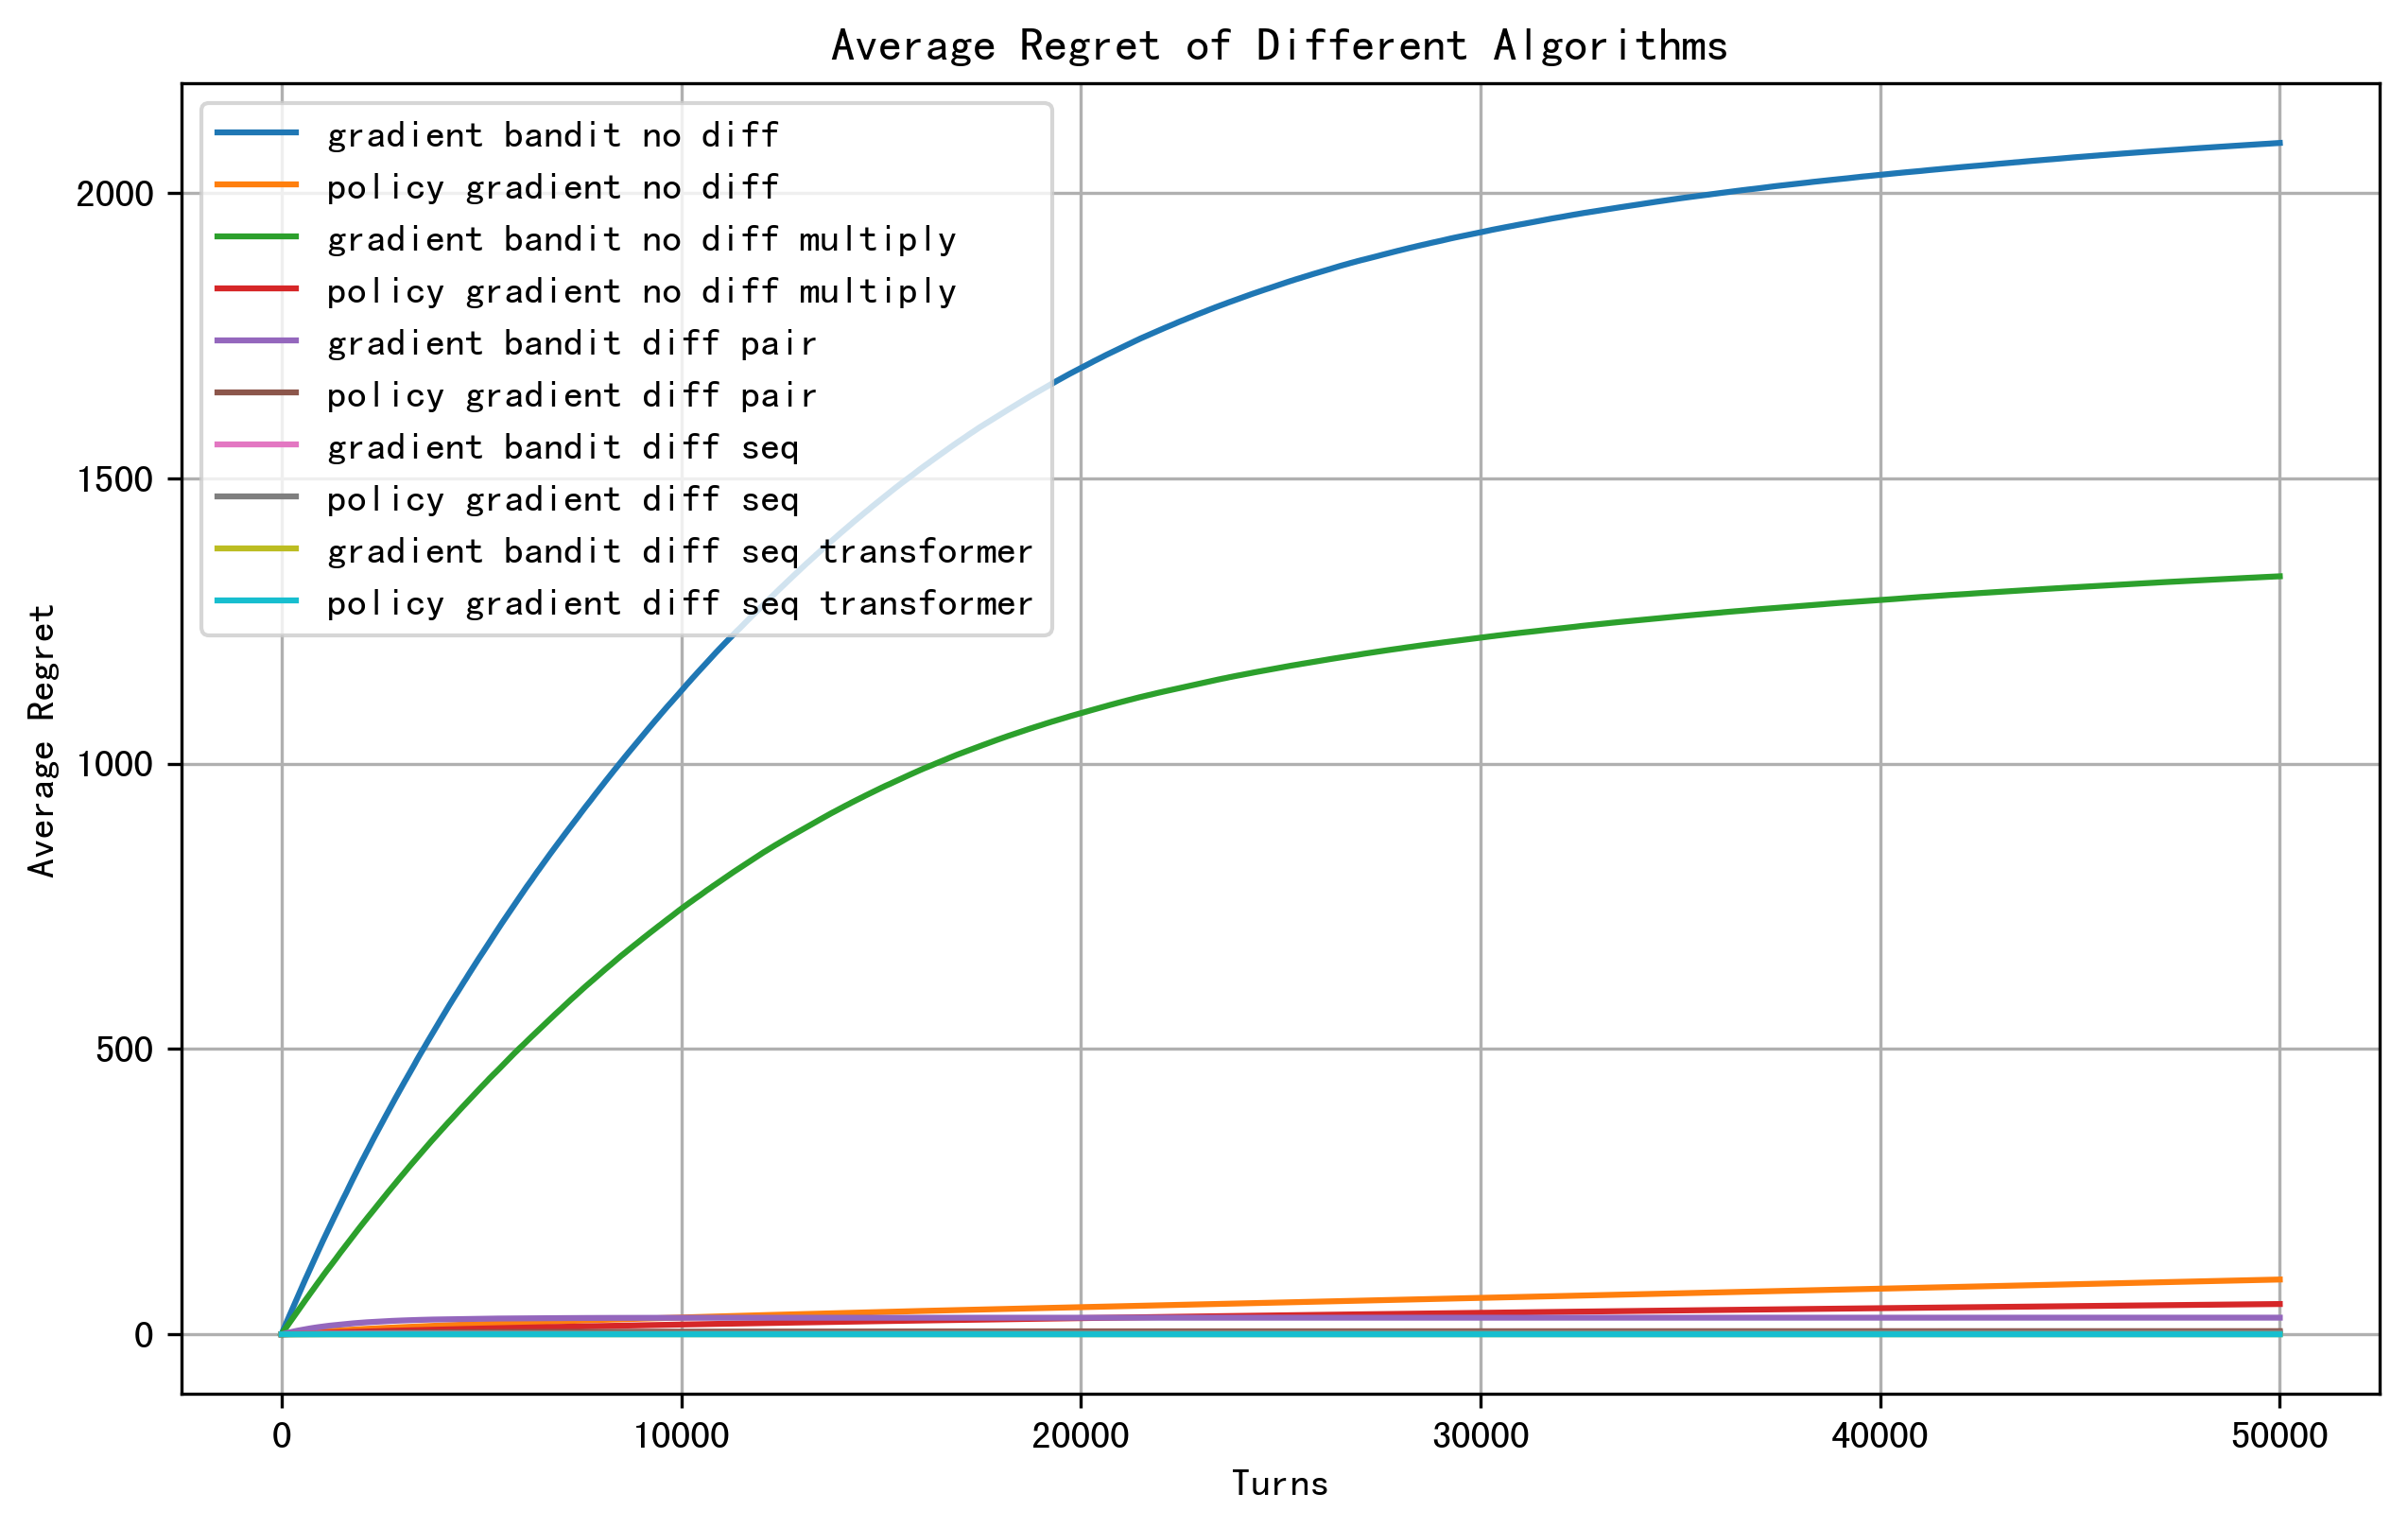
\includegraphics[width=0.9\textwidth]{./Img/stochastic_bandit/compare_gradient_bandit.png}
    \caption{Average cumulative-regret curves for the policy-gradient algorithm (Policy Gradient) and the gradient-bandit algorithm (Gradient Bandit) under five data regimes: the raw offline dataset without augmentation (no diff), the original dataset duplicated and concatenated (no diff multiply), tuple-level discrete diffusion augmentation (diff pair), sequential discrete diffusion augmentation (diff seq), and Transformer-based sequential discrete diffusion augmentation (diff seq transformer).}
    \label{fig:compare_gradient_bandit}
\end{figure}

\begin{table}[htbp]
    \centering
    \begin{tabular}{c c c}
    \toprule
    Trajectory generation policy & policy gradient & gradient bandit \\
    \midrule
    offline, no enlarge & 96.010 & 2078.776 \\
    offline+copy & 53.095 & 1316.211 \\
    offline+diffuse pair & 5.500 & 34.418 \\
    offline+diffusion sequence & 2.629 & 1.712 \\
    offline+diffusion sequence (Transformer) & 0.001 & 0.140 \\
    \bottomrule
\end{tabular}
\caption{Performance(average accumulated regret) of various algorithms on Bernoulli-reward bandits under different offline-dataset enlargement (trajectory-generation) policies.}
\label{table:compare_gradient_bandit}
\end{table}

Additionally, to confirm that the generated trajectories accurately capture the true distribution, we plot in Figure \ref{fig:distribution} both the number of times each arm is selected and each arm’s average observed reward. Because arms with higher indices have larger expected rewards in our setting, they are sampled more frequently, as expected. Moreover, the empirical mean reward for each arm closely matches its true expectation, demonstrating the effectiveness of our trajectory‐generation method.

\begin{figure}[htbp]
    \centering
    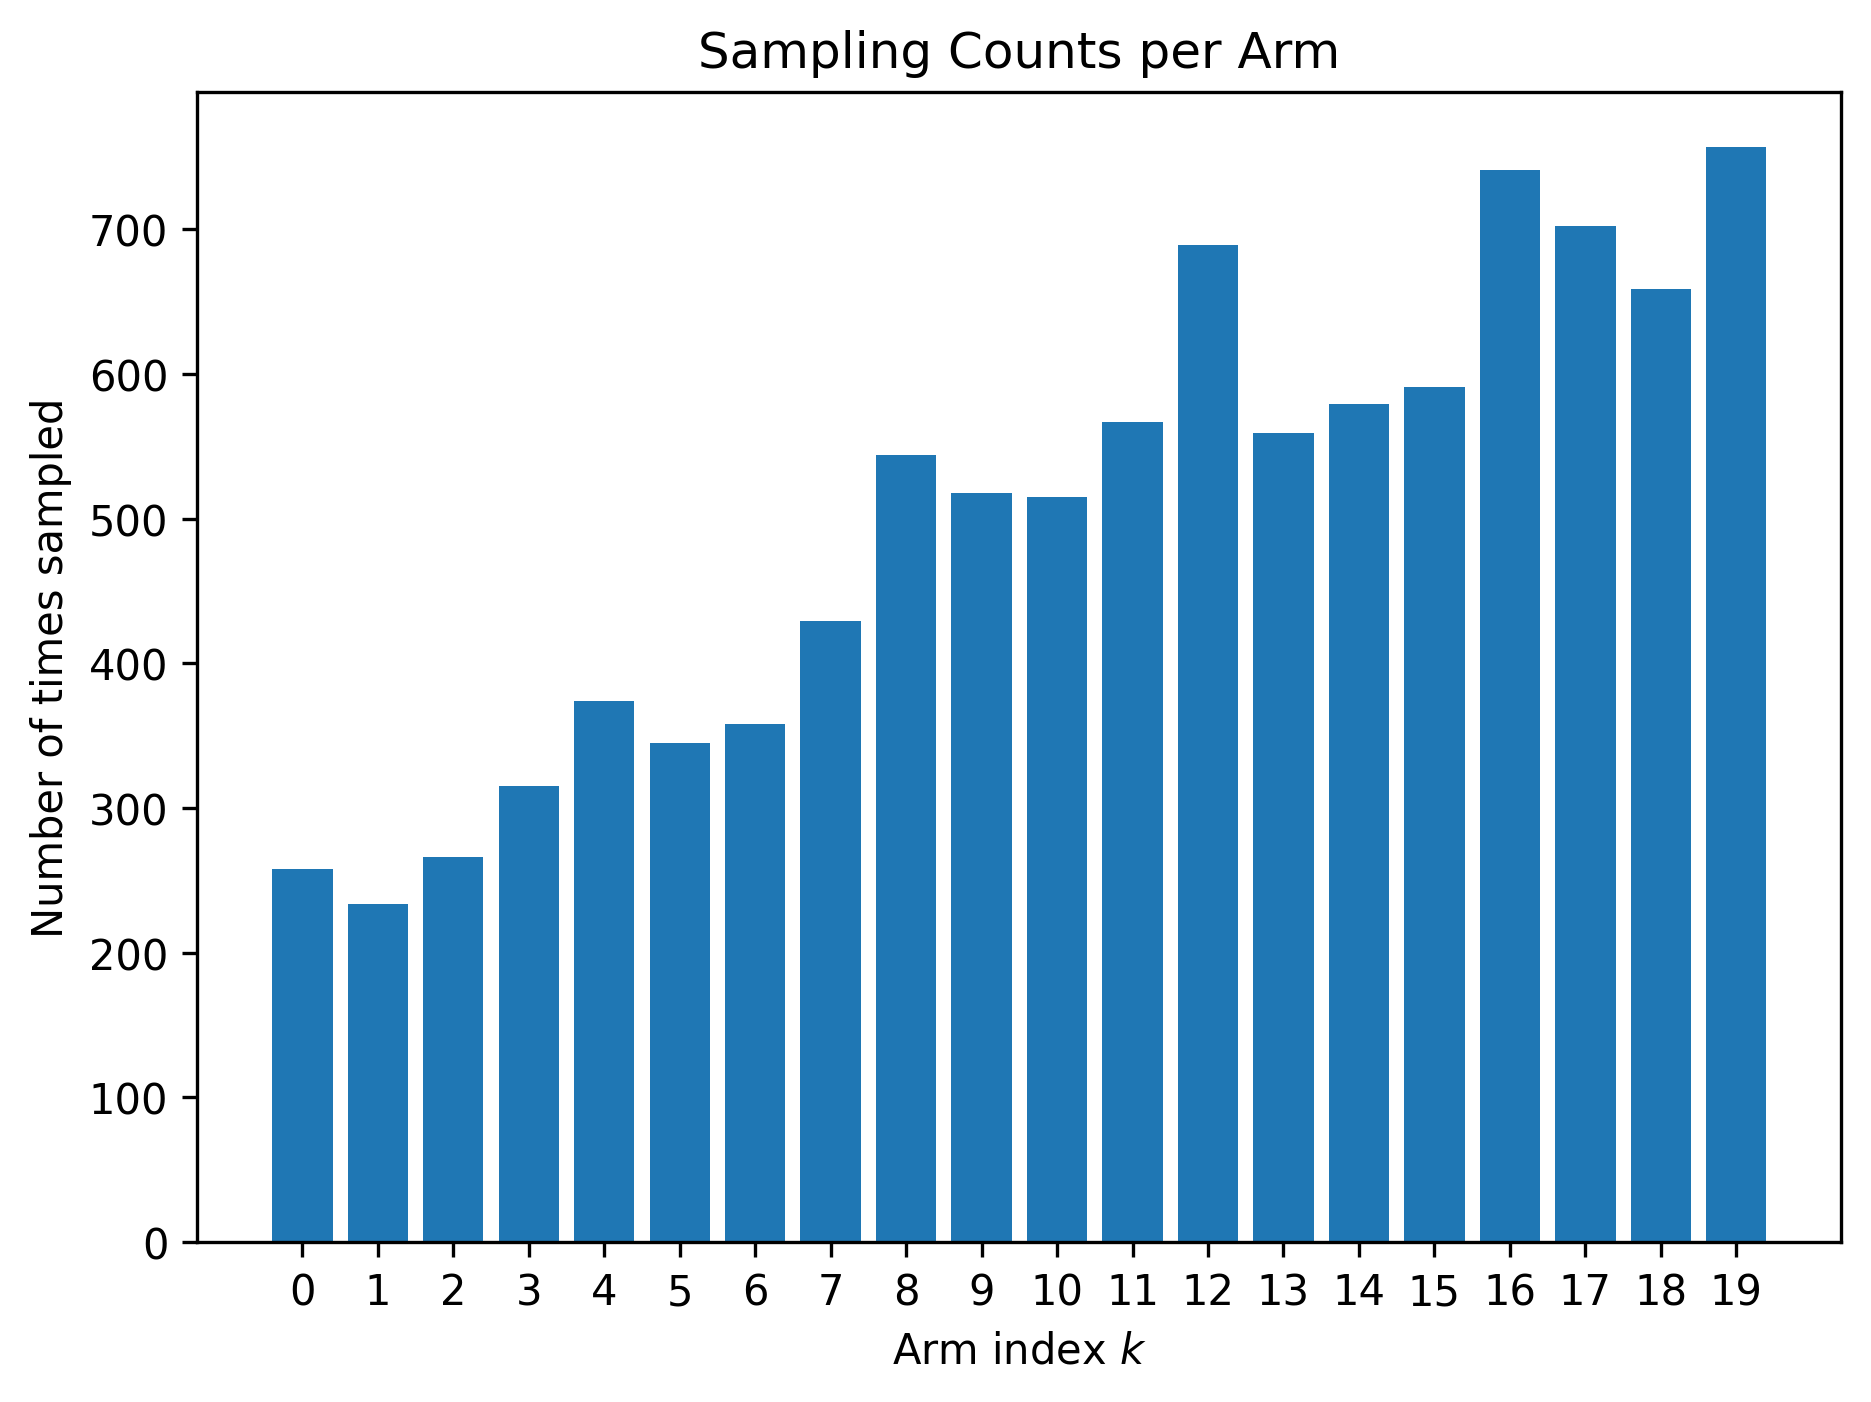
\includegraphics[width=0.48\textwidth]{./Img/stochastic_bandit/count.png}
    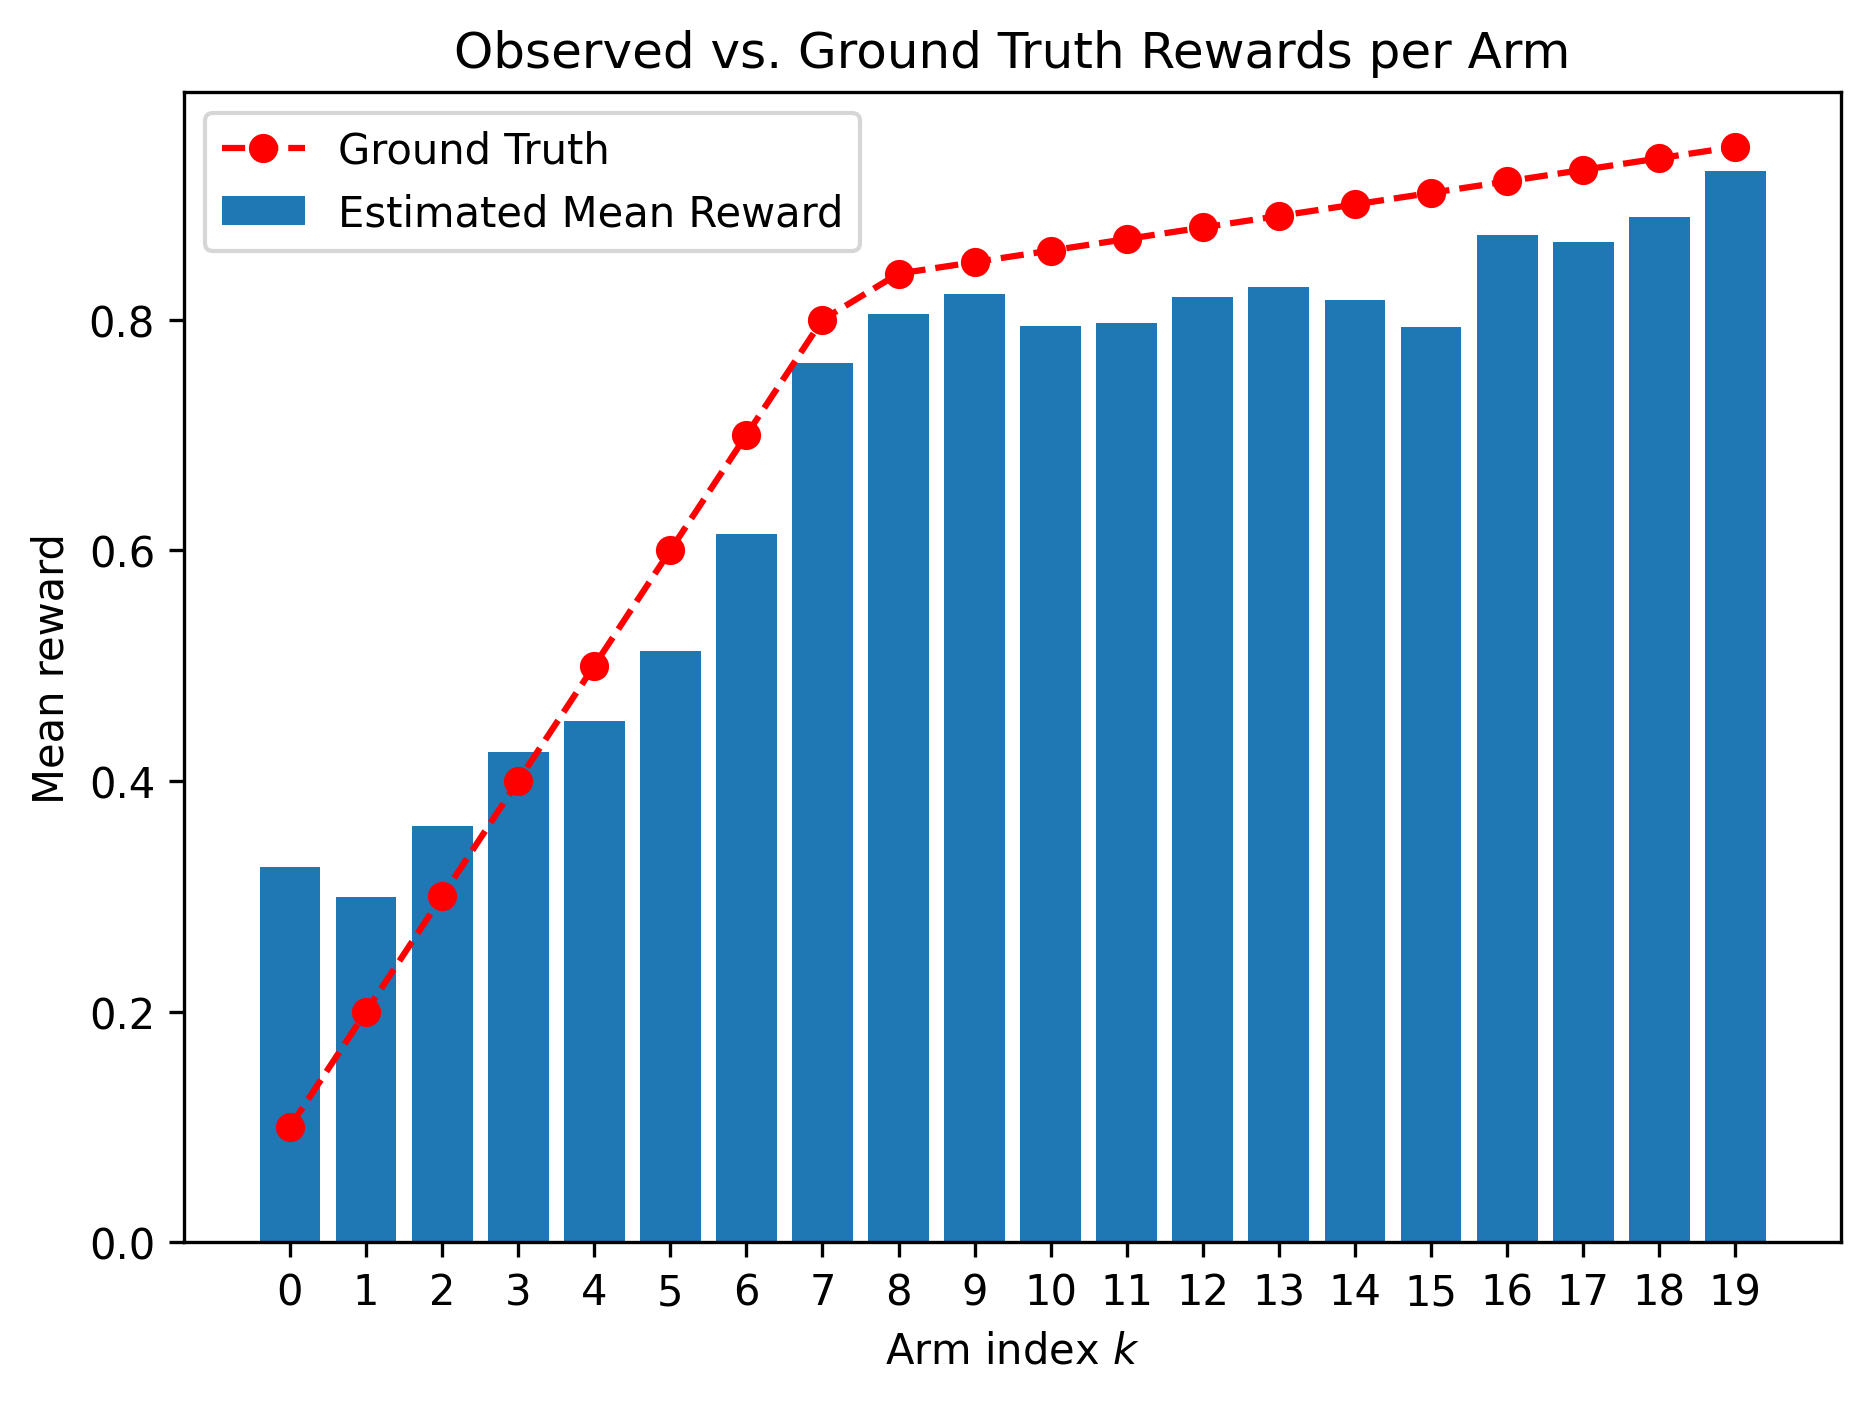
\includegraphics[width=0.48\textwidth]{./Img/stochastic_bandit/reward.png}
    \caption{Left: number of times each arm was selected in the generated trajectories. Right: empirical mean reward for each arm (blue bars) versus its true expected reward (red dashed line).}
    \label{fig:distribution}
\end{figure}


\subsection{contextual Bandit}

\begin{figure}[H]
    \centering
    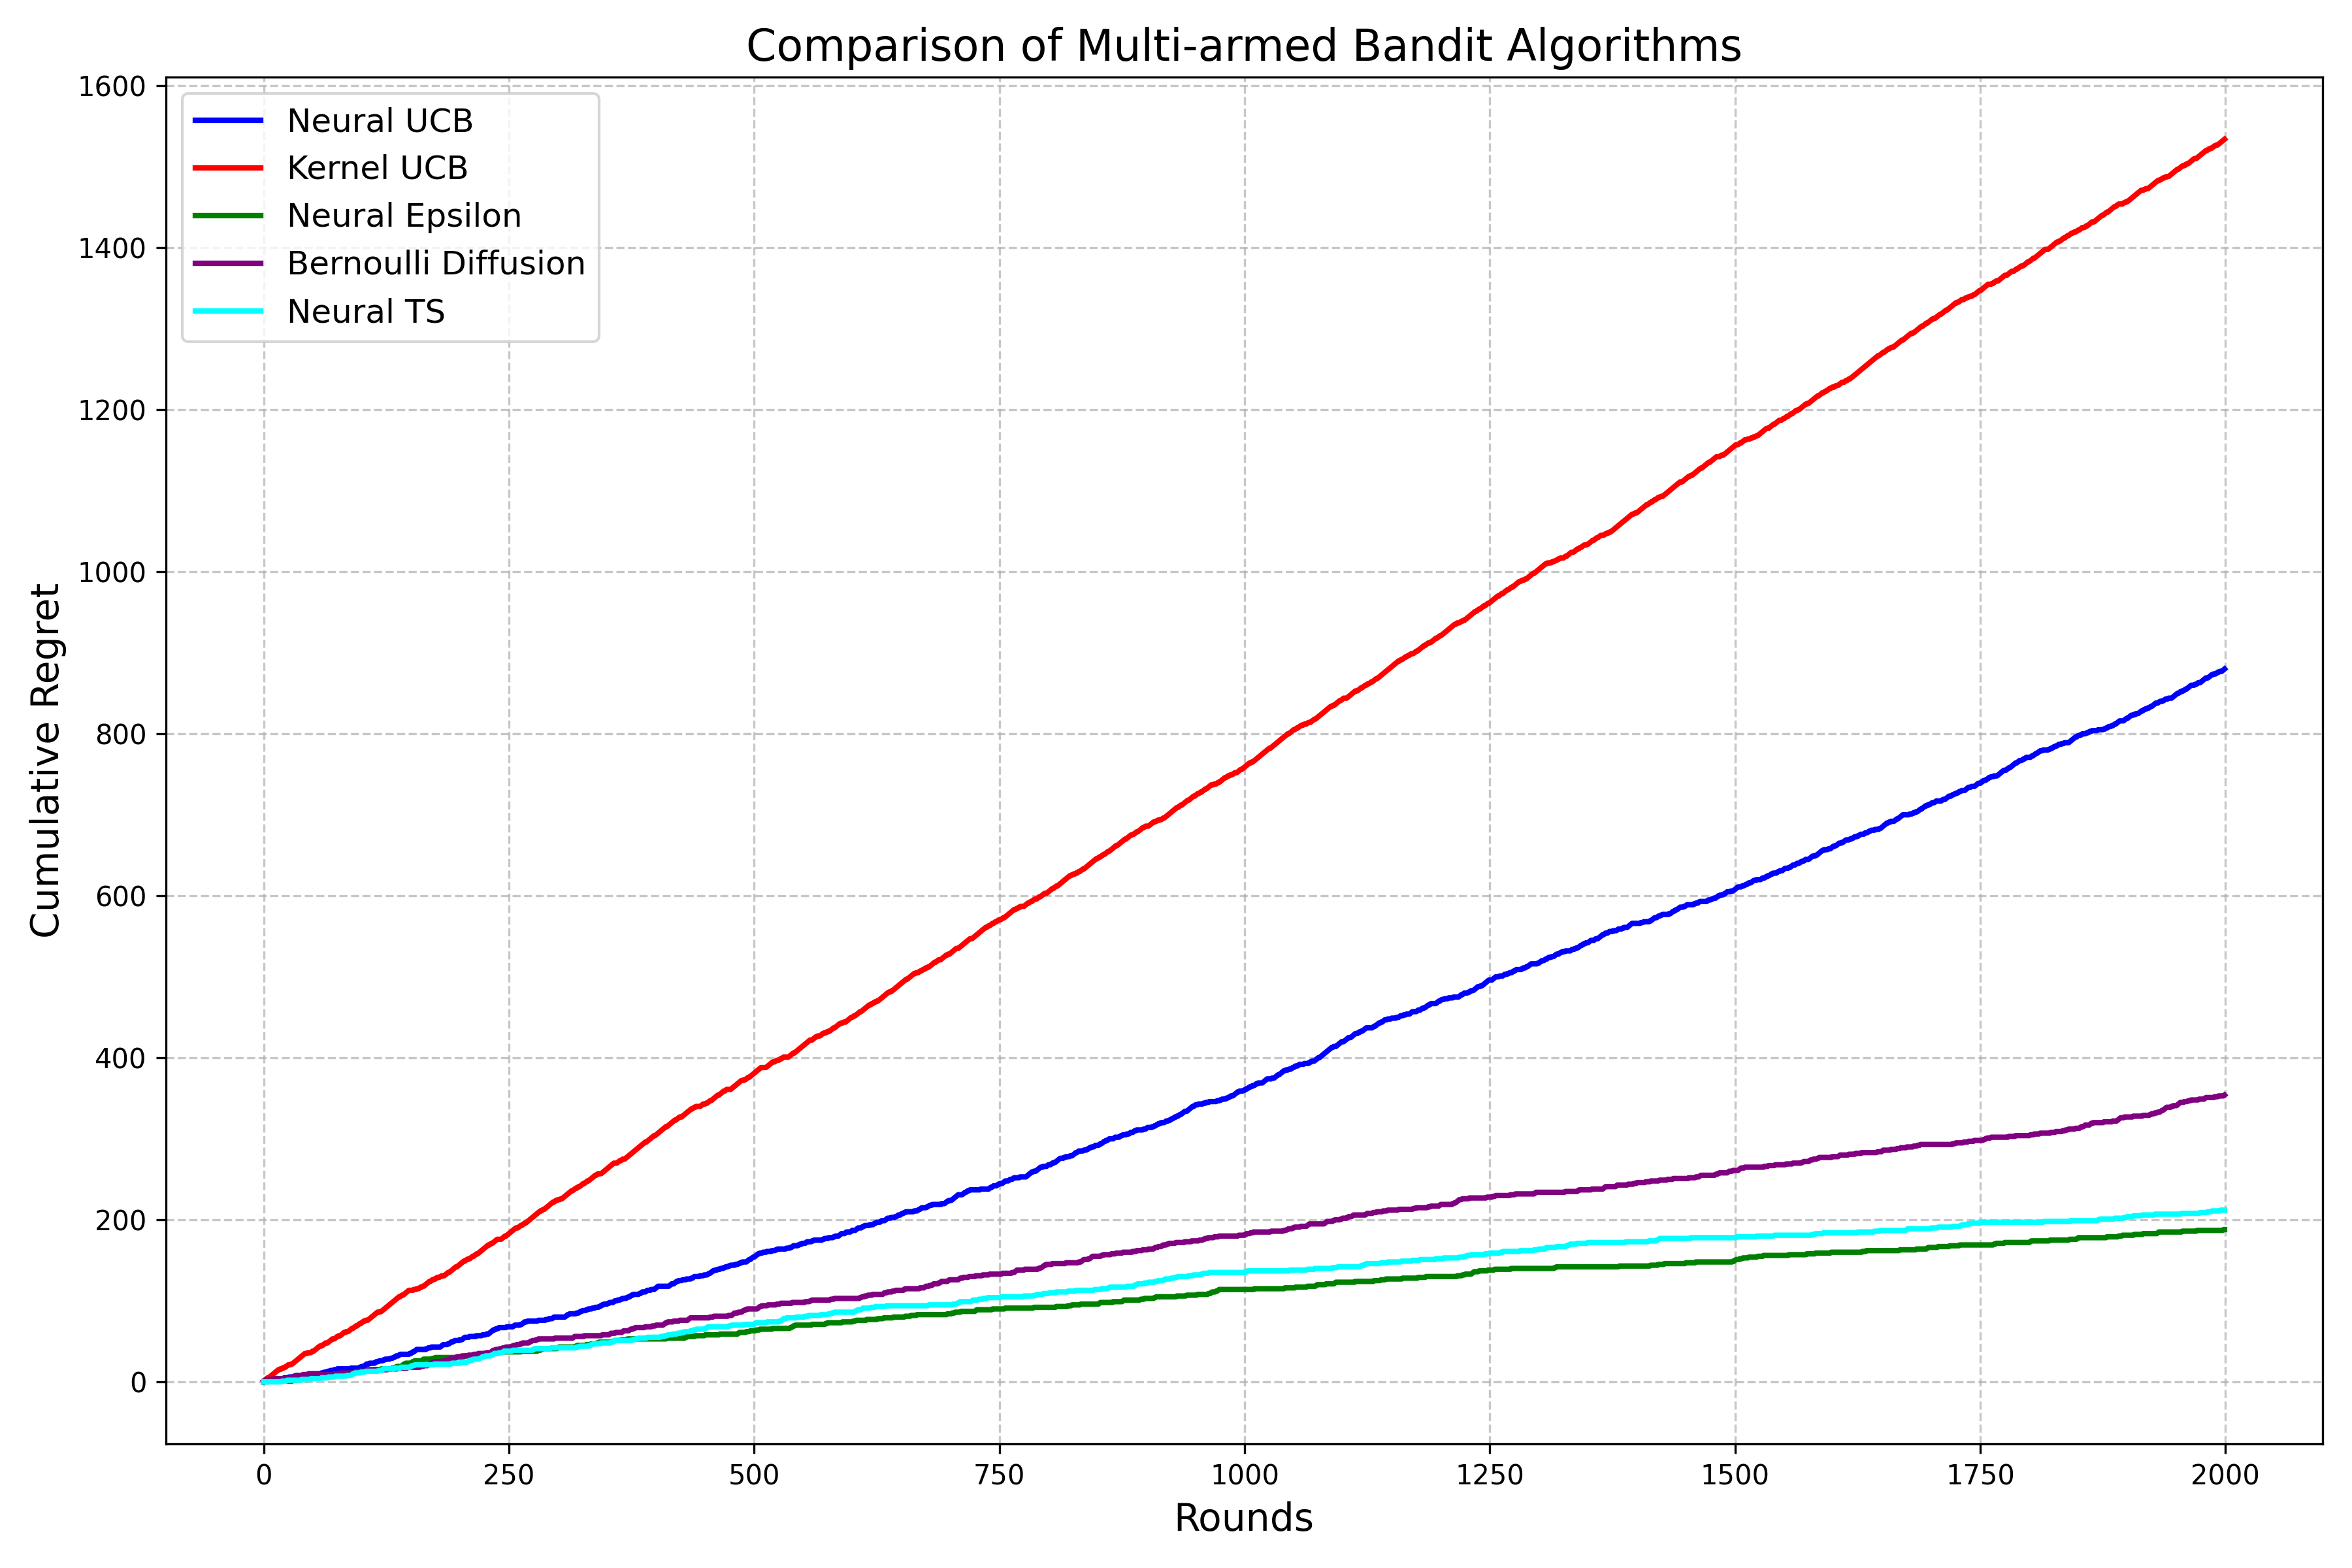
\includegraphics[width=0.9\linewidth]{Img/context_compare.png}
    \caption{Comparison of cumulative regret across different algorithms after 25 rounds of pertaining using the MNIST Dataset.}
    \label{fig:context_regret}
\end{figure}

\paragraph{Setup}
We evaluate our method on a contextual bandit task derived from MNIST, where each arm corresponds to a digit label. 
All models are pretrained on 3{,}000 offline samples for 25 epochs. Our method uses a conditional discrete diffusion model with a single denoising step. Evaluation is conducted over 2{,}000 online rounds, and performance is measured via cumulative regret.
We compare against \textbf{NeuralTS}, \textbf{Neural} $\boldsymbol{\varepsilon}$\textbf{-Greedy}, \textbf{NeuralUCB}, and \textbf{KernelUCB}. All methods share the same network architecture and training data. NeuralTS and $\varepsilon$-Greedy follow standard implementations from prior work.

\paragraph{Results}
As shown in Figure~\ref{fig:context_regret}, \textbf{Bernoulli Diffusion} outperforms UCB-based methods but underperforms NeuralTS and $\varepsilon$-Greedy. This suggests that while diffusion-based models can effectively learn conditional reward distributions and yield competitive performance, their stochastic nature may introduce unnecessary variance in binary-reward settings, where mean estimation is often sufficient. 
The uncertainty captured by the diffusion model does not yield improved decision quality and instead increases variance in action selection.



\section{Conclusion} \label{sec:5_conclusion}

\paragraph{Stochastic Bandit}

This study presents a stochastic multi-armed bandit algorithm based on policy gradients, augmented with a discrete diffusion model to generate offline trajectory data and thereby enrich a limited dataset. We conduct a comprehensive simulation by varying multiple factors—source of offline data, reward distributions per arm (Bernoulli vs. non-Bernoulli), trajectory-generation strategies, and the number of trajectories. Results show that, regardless of whether the rewards follow a Bernoulli or a non-Bernoulli distribution, the policy-gradient approach delivers strong performance in stochastic bandit environments. Moreover, when the offline dataset—initially collected with UCB or Thompson Sampling—is enhanced by diffusion-generated trajectories, the final average regret is substantially reduced.

Our experiments further demonstrate that incorporating temporal structure, particularly via a Transformer-based discrete diffusion model, more effectively captures sequential and time-series patterns in the data, producing trajectories that closely match those generated by the true policy. As the number of diffusion-generated trajectories increases, the benefits of pre-training become even more pronounced, revealing excellent scalability and generalization ability.

In summary, the proposed Transformer-based discrete diffusion trajectory generation method yields significant pre-training advantages in stochastic multi-armed bandit problems. It not only mitigates sample scarcity during policy learning but also markedly lowers average regret, offering a practical and efficient solution for policy optimization in offline reinforcement learning settings.


\paragraph{Contextual Bandit}

We presented a diffusion-based approach to contextual bandits that models the full conditional reward distribution instead of relying solely on mean estimation. While our method performs competitively and outperforms several UCB-based baselines, it underperforms compared to simpler mean-based strategies such as NeuralTS and $\varepsilon$-Greedy in binary reward settings. This highlights a trade-off: the expressive power of distributional modeling may be underutilized when the reward structure is simple.
Looking forward, we plan to design contextual bandit environments with richer reward distributions, e.g., bimodal or heavy-tailed, where capturing higher-order uncertainty is essential. Such settings will better showcase the potential of diffusion-based methods in modeling complex decision uncertainty beyond mean reward estimates.


\newpage
{
    \small
    \bibliographystyle{unsrt}
    \bibliography{section/reference}
}

\end{document}